% TO-DO:
% * slides to mention big achievements, 附件

\documentclass[16pt]{beamer}

\ifdefined\chinchin
\usepackage[CJKspace]{xeCJK}
%\setCJKmainfont[BoldFont=SimHei,ItalicFont=AR PL KaitiM GB]{Alibaba PuHuiTi}
\setCJKmainfont{Alibaba PuHuiTi}
\newcommand{\cc}[2]{#1}
\else
\newcommand{\cc}[2]{#2}
\renewcommand{\baselinestretch}{0.8} 
\fi

%\usepackage{newtxtext,newtxmath}	% use Times Roman font
%\usepackage{newtxtext}
%\renewcommand{\familydefault}{\sfdefault}
\usefonttheme{serif}
\usefonttheme{professionalfonts}
%\setbeamertemplate{theorems}[numbered]
\setbeamertemplate{caption}{\insertcaption} 	% no `Figure' prefix before caption

\mode<presentation> {

%\usetheme{default}
%\usetheme{AnnArbor}
%\usetheme{Antibes}
%\usetheme{Bergen}
%\usetheme{Berkeley}
%\usetheme{Berlin}
%\usetheme{Boadilla}
%\usetheme{CambridgeUS}
%\usetheme{Copenhagen}
%\usetheme{Darmstadt}
%\usetheme{Dresden}
%\usetheme{Frankfurt}
%\usetheme{Goettingen}
%\usetheme{Hannover}
%\usetheme{Ilmenau}
%\usetheme{JuanLesPins}
%\usetheme{Luebeck}
\usetheme{Madrid}
%\usetheme{Malmoe}
%\usetheme{Marburg}
%\usetheme{Montpellier}
%\usetheme{PaloAlto}
%\usetheme{Pittsburgh}
%\usetheme{Rochester}
%\usetheme{Singapore}
%\usetheme{Szeged}
%\usetheme{Warsaw}

%\usecolortheme{albatross}
%\usecolortheme{beaver}
%\usecolortheme{beetle}
%\usecolortheme{crane}
%\usecolortheme{dolphin}
%\usecolortheme{dove}
%\usecolortheme{fly}
%\usecolortheme{lily}
\usecolortheme{orchid}
%\usecolortheme{rose}
%\usecolortheme{seagull}
%\usecolortheme{seahorse}
%\usecolortheme{whale}
%\usecolortheme{wolverine}		% Hofstra

%\setbeamertemplate{footline} % To remove the footer line in all slides uncomment this line
\setbeamertemplate{footline}[page number] % To replace the footer line in all slides with a simple slide count uncomment this line
\setbeamertemplate{navigation symbols}{} % To remove the navigation symbols from the bottom of all slides uncomment this line
}

\setbeamertemplate{headline}{}
\setbeamersize{text margin left=1mm,text margin right=1mm} 
\settowidth{\leftmargini}{\usebeamertemplate{itemize item}}
\addtolength{\leftmargini}{\labelsep}

\usepackage[backend=biber,style=numeric]{biblatex}
\bibliography{../AGI-book}
% \renewcommand*{\bibfont}{\footnotesize}
\setbeamertemplate{bibliography item}[text]

\usepackage{graphicx} % Allows including images
\usepackage{tikz-cd}
\usepackage{tikz}
\usepackage[export]{adjustbox}% http://ctan.org/pkg/adjustbox
\usepackage{verbatim} % comments
% \usepackage{tikz-cd}  % commutative diagrams
% \newcommand{\tikzmark}[1]{\tikz[overlay,remember picture] \node (#1) {};}
% \usepackage{booktabs} % Allows the use of \toprule, \midrule and \bottomrule in tables
% \usepackage{amssymb}  % \leftrightharpoons
% \usepackage{wasysym} % frownie face
% \usepackage{newtxtext,newtxmath}	% Times New Roman font
% \usepackage{sansmath}

\newcommand{\emp}[1]{\textbf{\color{violet}#1}}
\newcommand{\vect}[1]{\boldsymbol{#1}}
\newcommand{\tab}{\hspace*{1cm}}
\newcommand*\confoundFace{$\vcenter{\hbox{\includegraphics[scale=0.2]{../confounded-face.jpg}}}$}
\newcommand{\smiley}{$\vcenter{\hbox{\includegraphics[scale=0.05]{../smiling-face.png}}}$}

\makeatletter
\renewcommand{\boxed}[1]{\fbox{\m@th$\displaystyle\scalebox{0.9}{#1}$} \,}
\makeatother

%%%%%%%% Make table of contents %%%%%%%

\newif\ifframeinlbf
\frameinlbftrue
\makeatletter
\newcommand\listofframes{\@starttoc{lbf}}
\makeatother
\addtobeamertemplate{frametitle}{}{%
	\ifframeinlbf
	\addcontentsline{lbf}{section}{\protect\makebox[2em][l]{%
			\protect\usebeamercolor[fg]{structure}\insertframenumber\hfill}%
		\insertframetitle\par}%
	\else\fi
}

%%%%%%%% Include Parts in TOC %%%%%%%

\makeatletter
\AtBeginPart{%
	\addtocontents{toc}{\protect\beamer@partintoc{\the\c@part}{\beamer@partnameshort}{\the\c@page}}%
}
%% number, shortname, page.
\providecommand\beamer@partintoc[3]{%
	\ifnum\c@tocdepth=-1\relax
	% requesting onlyparts.
	\makebox[6em]{PART #1:} #2
	\par
	\fi
}
\define@key{beamertoc}{onlyparts}[]{%
	\c@tocdepth=-1\relax
}
\makeatother%

%----------------------------------------------------------------------------------------
%	TITLE PAGE
%----------------------------------------------------------------------------------------

\title[AGI via Logic]{{\Huge AGI via Combining Logic and Deep Learning}
 \\ \vspace*{0.4cm} AGI 2021 Conference}
\author{\cc{YKY}{YKY}} % Your name
%\institute[] % Your institution as it will appear on the bottom of every slide, may be shorthand to save space
%{
%Independent researcher, Hong Kong \\ % Your institution for the title page
%\medskip
%\textit{generic.intelligence@gmail.com} % Your email address
%}
\date{\today} % Date, can be changed to a custom date

\begin{document}

\frameinlbffalse
\addtocounter{page}{-1}
\begin{frame}[plain,noframenumbering]
\titlepage
\end{frame}

\addtocounter{page}{-1}
\begin{frame}[noframenumbering]
\frametitle{Table of contents}
\listofframes
% \vspace*{0.5cm}
% 多谢 支持 \smiley
\end{frame}

%----------------------------------------------------------------------------------------
%	PRESENTATION SLIDES
%----------------------------------------------------------------------------------------

%------------------------------------------------

\frameinlbftrue

\part{Categorical Logic}
\frame{\partpage}

\begin{frame}
\frametitle{Categorical Logic}
\begin{itemize}
	\item Quantifier as adjunctions
\end{itemize}
\end{frame}

\begin{frame}
\frametitle{Fibrations}
\begin{itemize}
	\item Fibration
\end{itemize}
\begin{equation}
\vcenter{\hbox{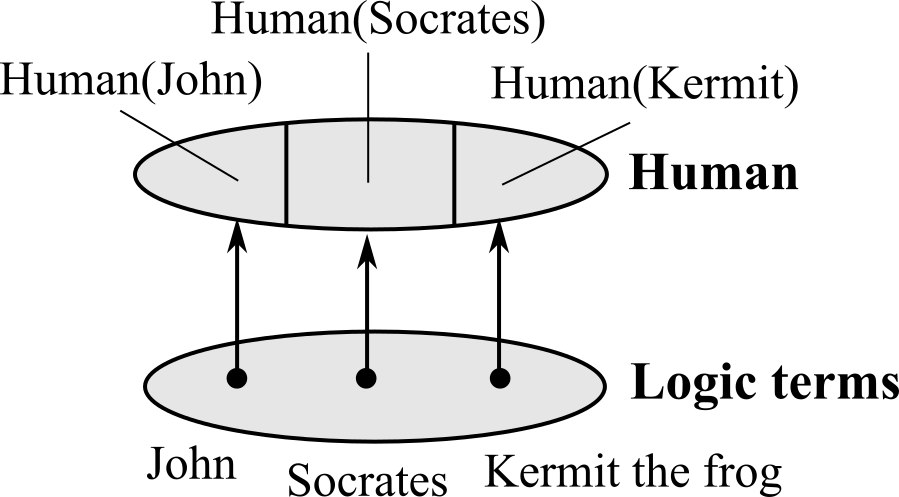
\includegraphics[scale=0.5]{dependent-type.png}}}
\nonumber
\end{equation}
\end{frame}

\part{Model-based vs Syntax-based}
\frame{\partpage}

\begin{frame}
\frametitle{Hitzler's Core Method}
\begin{itemize}
	\item The \textbf{semantic operator} $\mathcal{T}_P$ updates an interpretation to another interpretation:
\end{itemize}
\centering
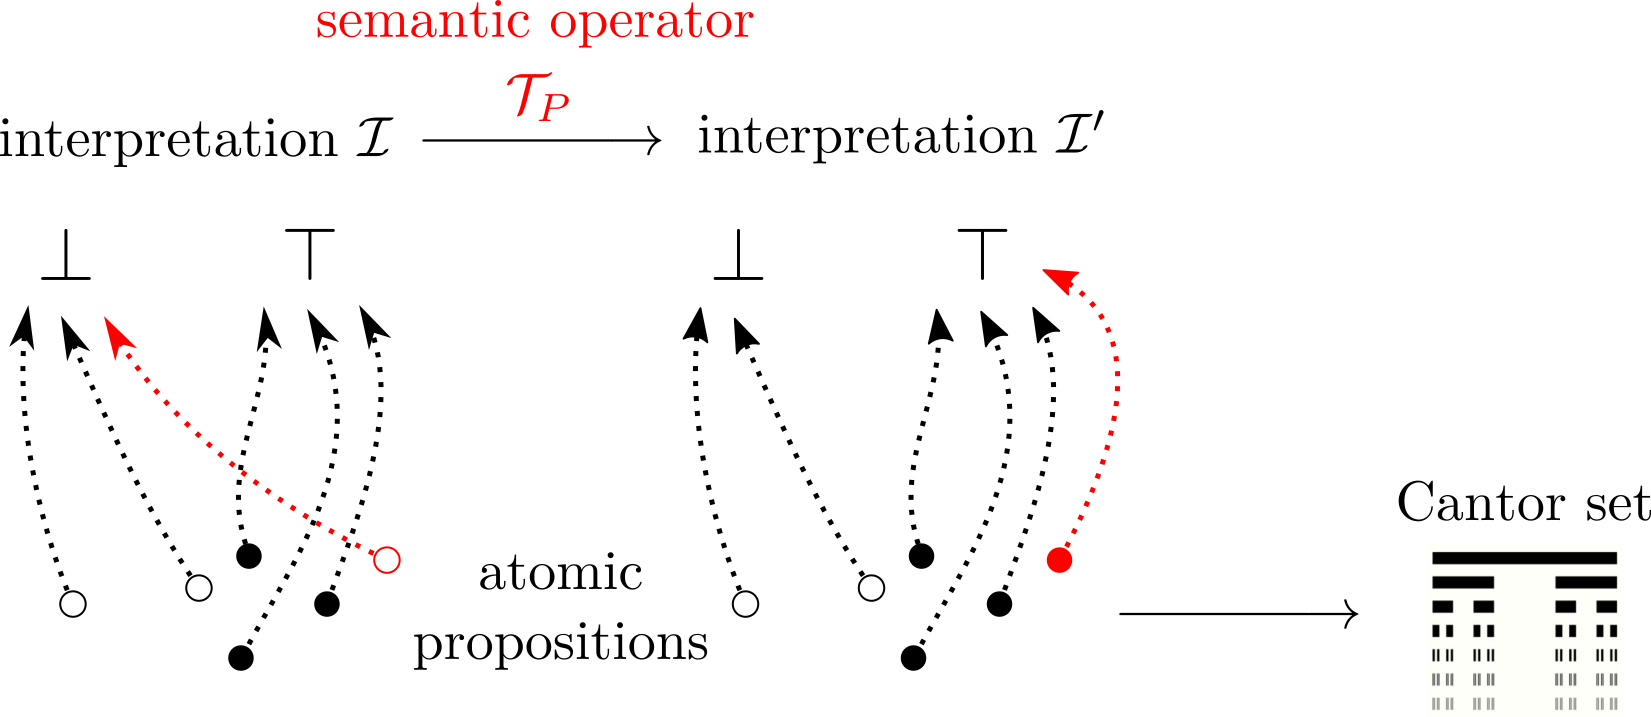
\includegraphics[scale=0.5]{Hitzler-semantic-operator.png}
\end{frame}

\begin{frame}
\frametitle{Hitzler's Core Method}
\begin{itemize}
	\item The \textbf{level mapping} $\iota$ takes an interpretation to a real number:
\end{itemize}
\begin{equation}
\vcenter{\hbox{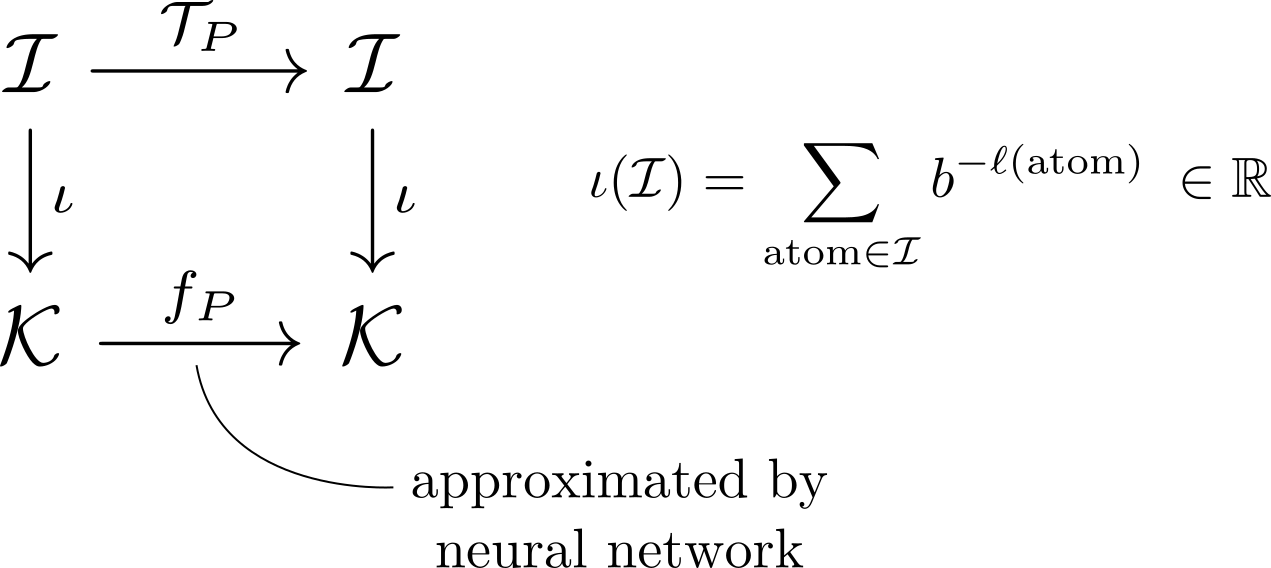
\includegraphics[scale=0.5]{Hitzler-level-mapping.png}}} \nonumber
\end{equation}
\end{frame}

\part{Reinforcement Learning}
\frame{\partpage}

\begin{frame}
\frametitle{This is a lamprey}
	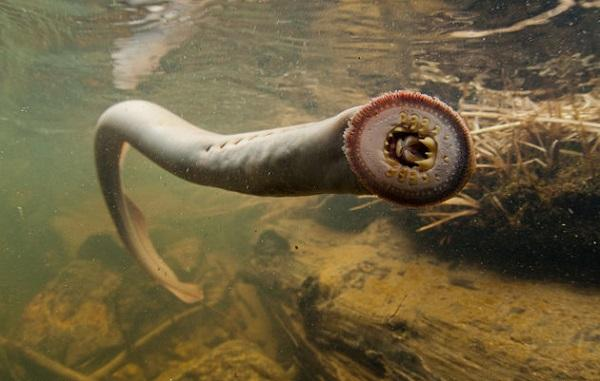
\includegraphics[scale=0.65]{lamprey.jpg}
\end{frame}

\begin{frame}
\frametitle{Evolution of the Neocortex}
\centering
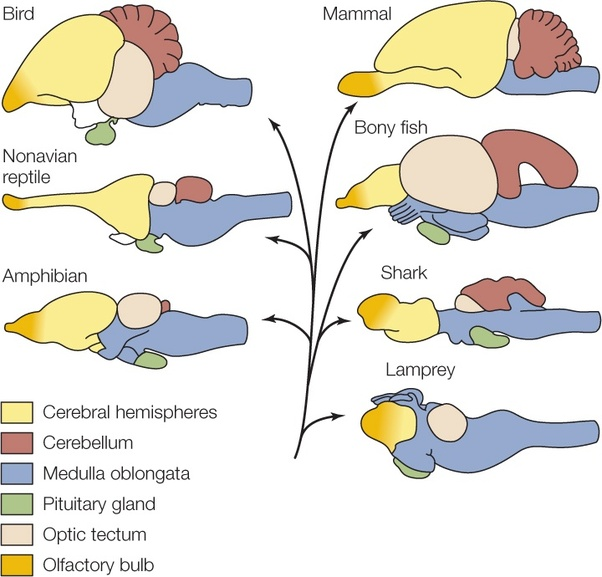
\includegraphics[scale=0.4]{lamprey-to-neocortex.jpg}
\end{frame}

\begin{frame}
\frametitle{Neocortex vs Reinforcement Learning}
\centering
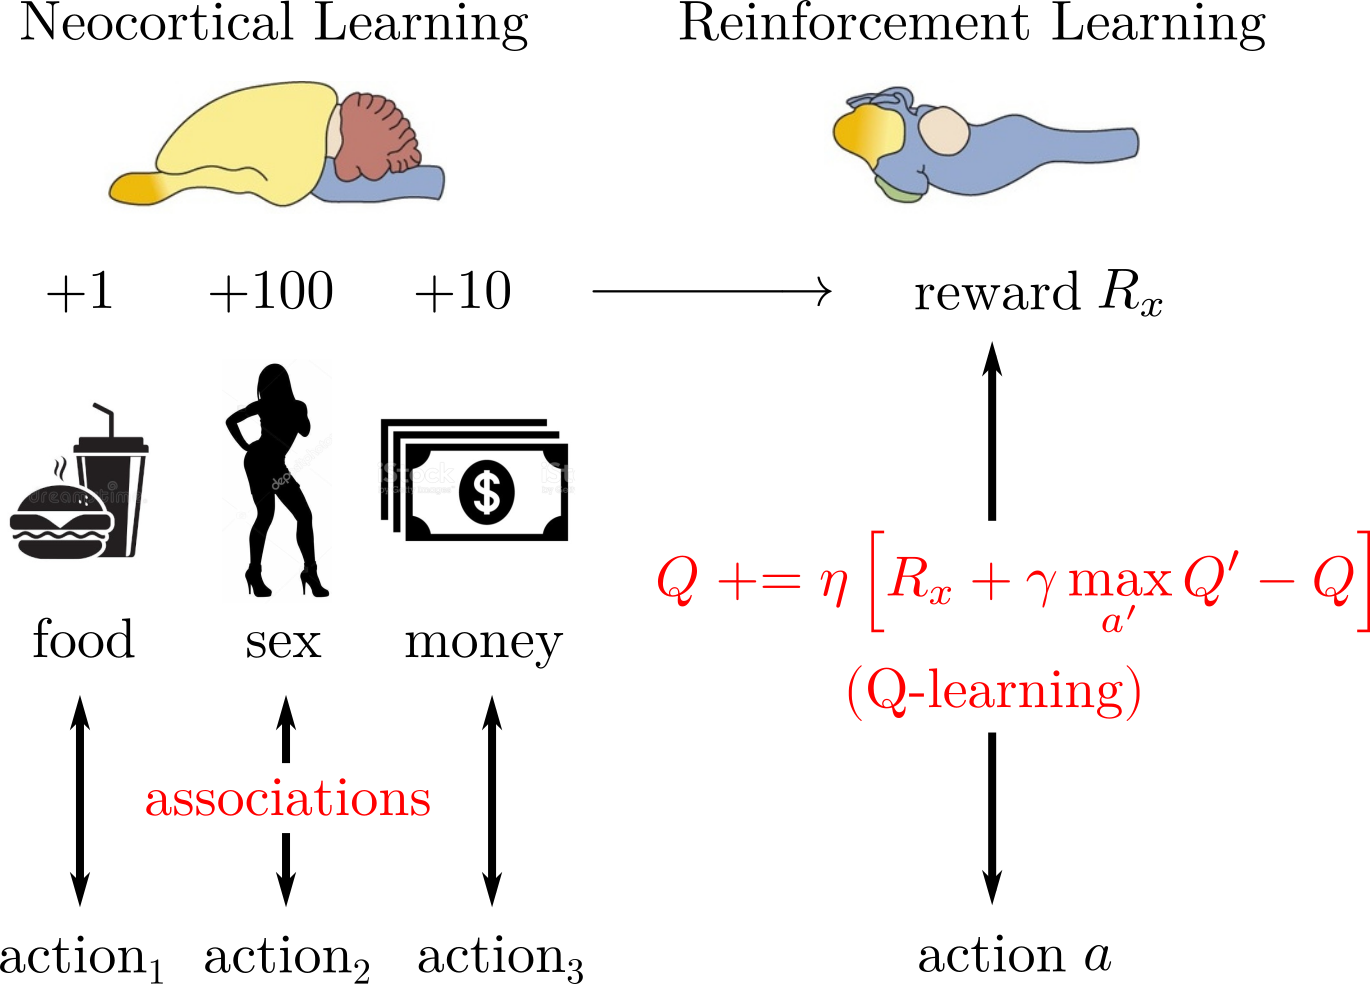
\includegraphics[scale=0.5]{neocortex-vs-RL.png}
\end{frame}

\part{BERT / GPT}
\frame{\partpage}

\begin{frame}
\frametitle{Equivariance of the Transformer}
\begin{itemize}
	\item Many people already know this: \\
	the Transformer module is \textbf{equivariant} in its inputs and outputs:
\end{itemize}
\centering
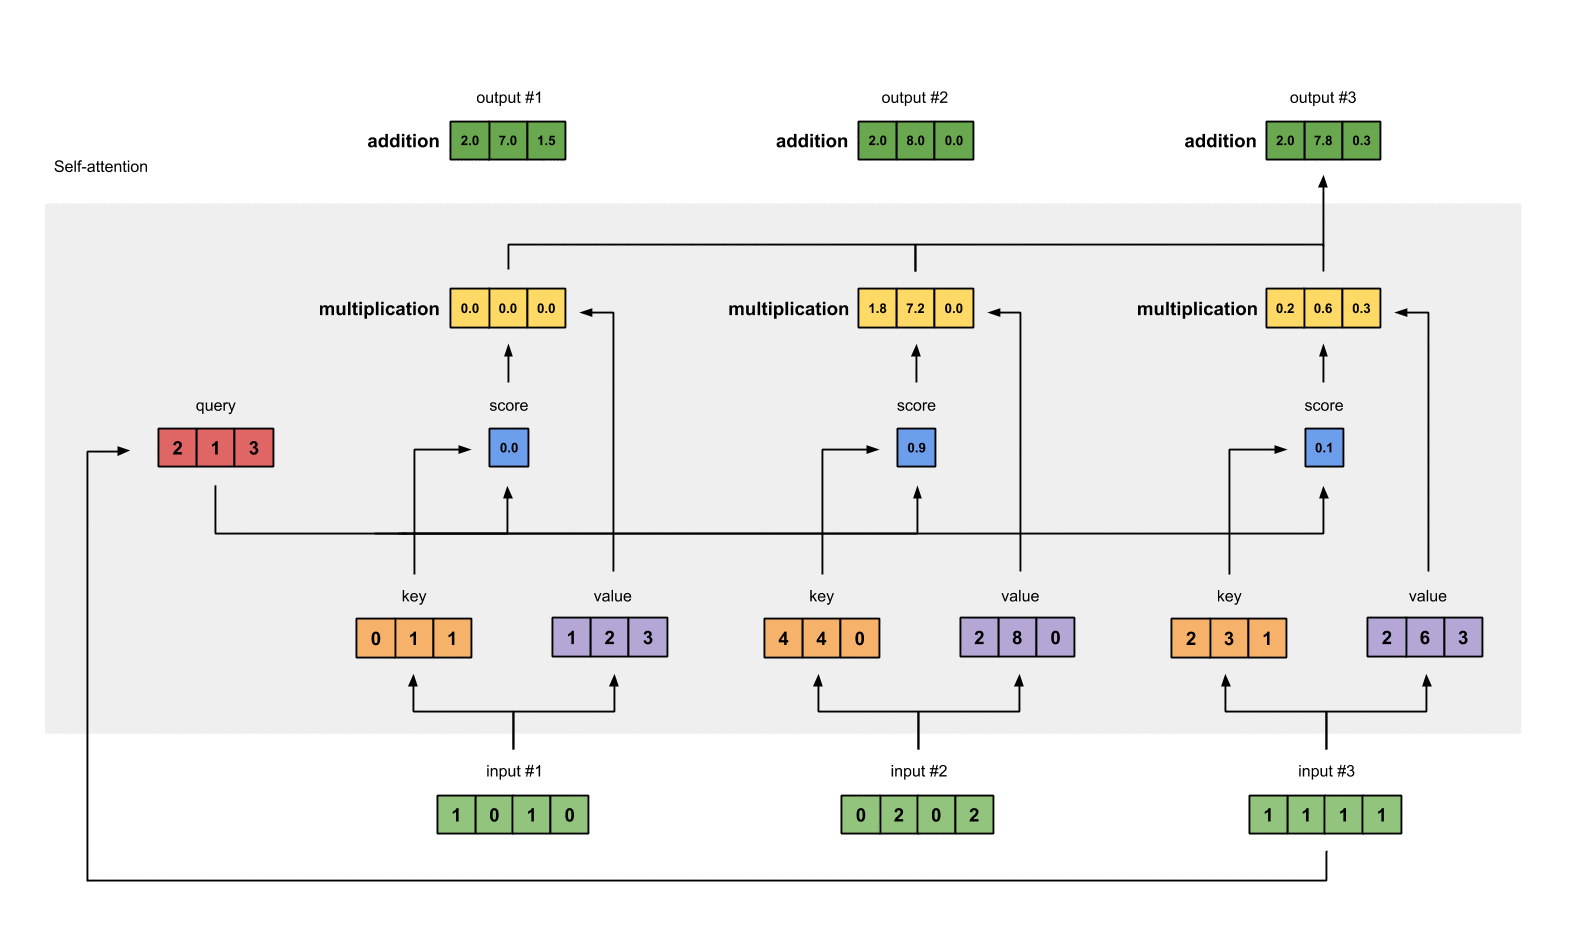
\includegraphics[scale=0.2]{self-attention.png}
\end{frame}

\begin{frame}
\frametitle{Additivity of Word Embeddings}
\centering
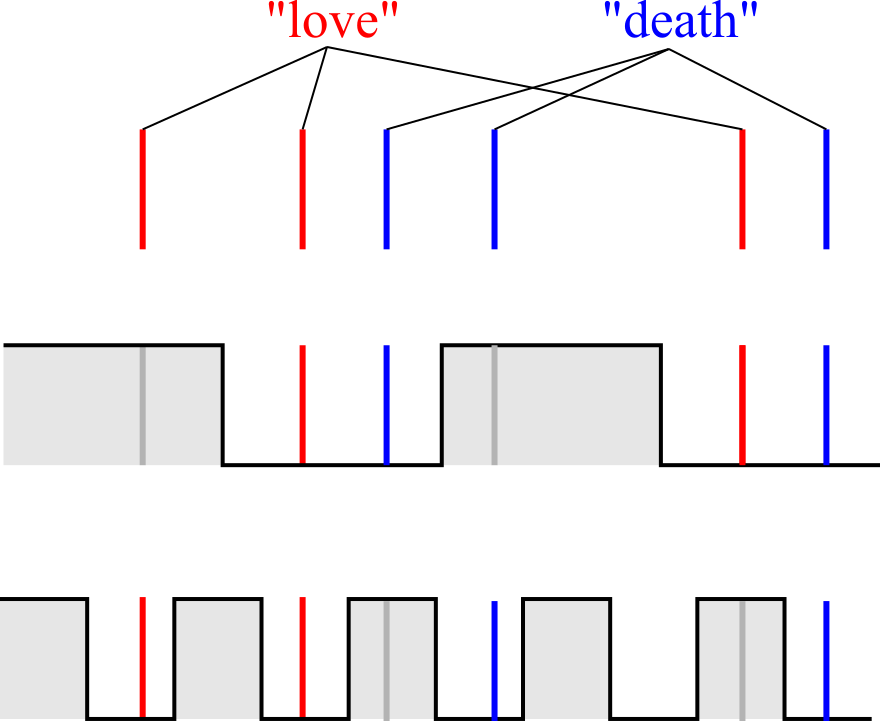
\includegraphics[scale=0.5]{positional-encoding.png}
\vspace*{1em}
\begin{itemize}
	\item This suggests that word embeddings can be added together to give \textbf{composite} meanings
\end{itemize}
\end{frame}

\begin{frame}
\frametitle{BERT's Hidden Representation}
\begin{itemize}
	\item This may be a close description of how BERT performs question-answering or logic deduction:
\end{itemize}
\vspace*{1em}
\centering
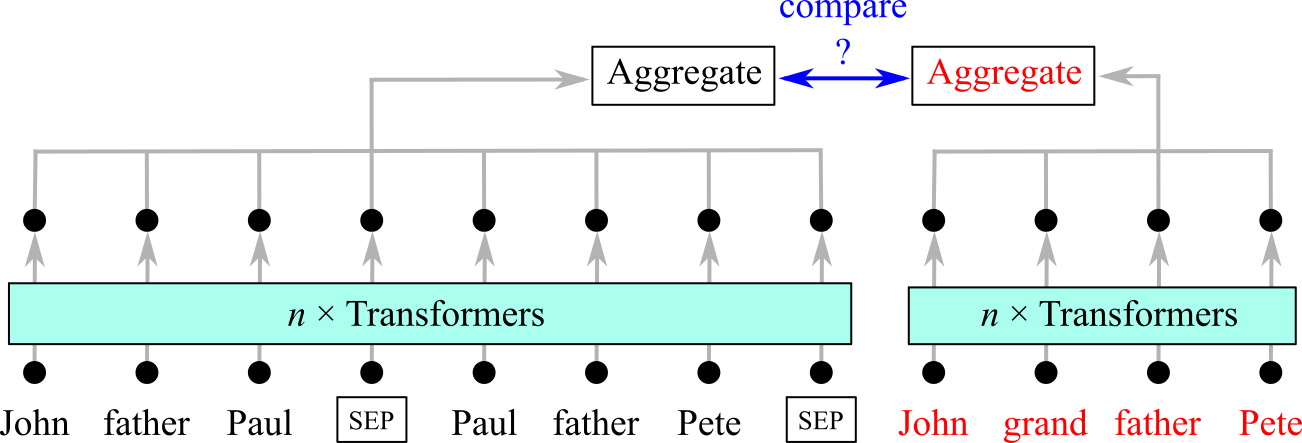
\includegraphics[scale=0.7]{Transformer-QnA.png}
\end{frame}

\part{BERT + Knowledge Graphs}
\frame{\partpage}

\begin{frame}
\frametitle{Memory Formation}
\begin{itemize}
	\item Memory
\end{itemize}
\end{frame}

\begin{frame}
\frametitle{Memory Recall}
\begin{itemize}
	\item Memory retrieval
\end{itemize}
\end{frame}

\part{Old Stuffs}
\frame{\partpage}

\begin{frame}
\frametitle{\cc{CNN 在机器视觉中的成功}{The success of CNN in computer vision}}
\begin{itemize}
	\item \cc{
	在几何学上,视觉 具有 \emp{平移 不变性}:}{
	In geometry, vision is said to possess the property of \textbf{translation invariance}:
	}
	\begin{equation}
	\vcenter{\hbox{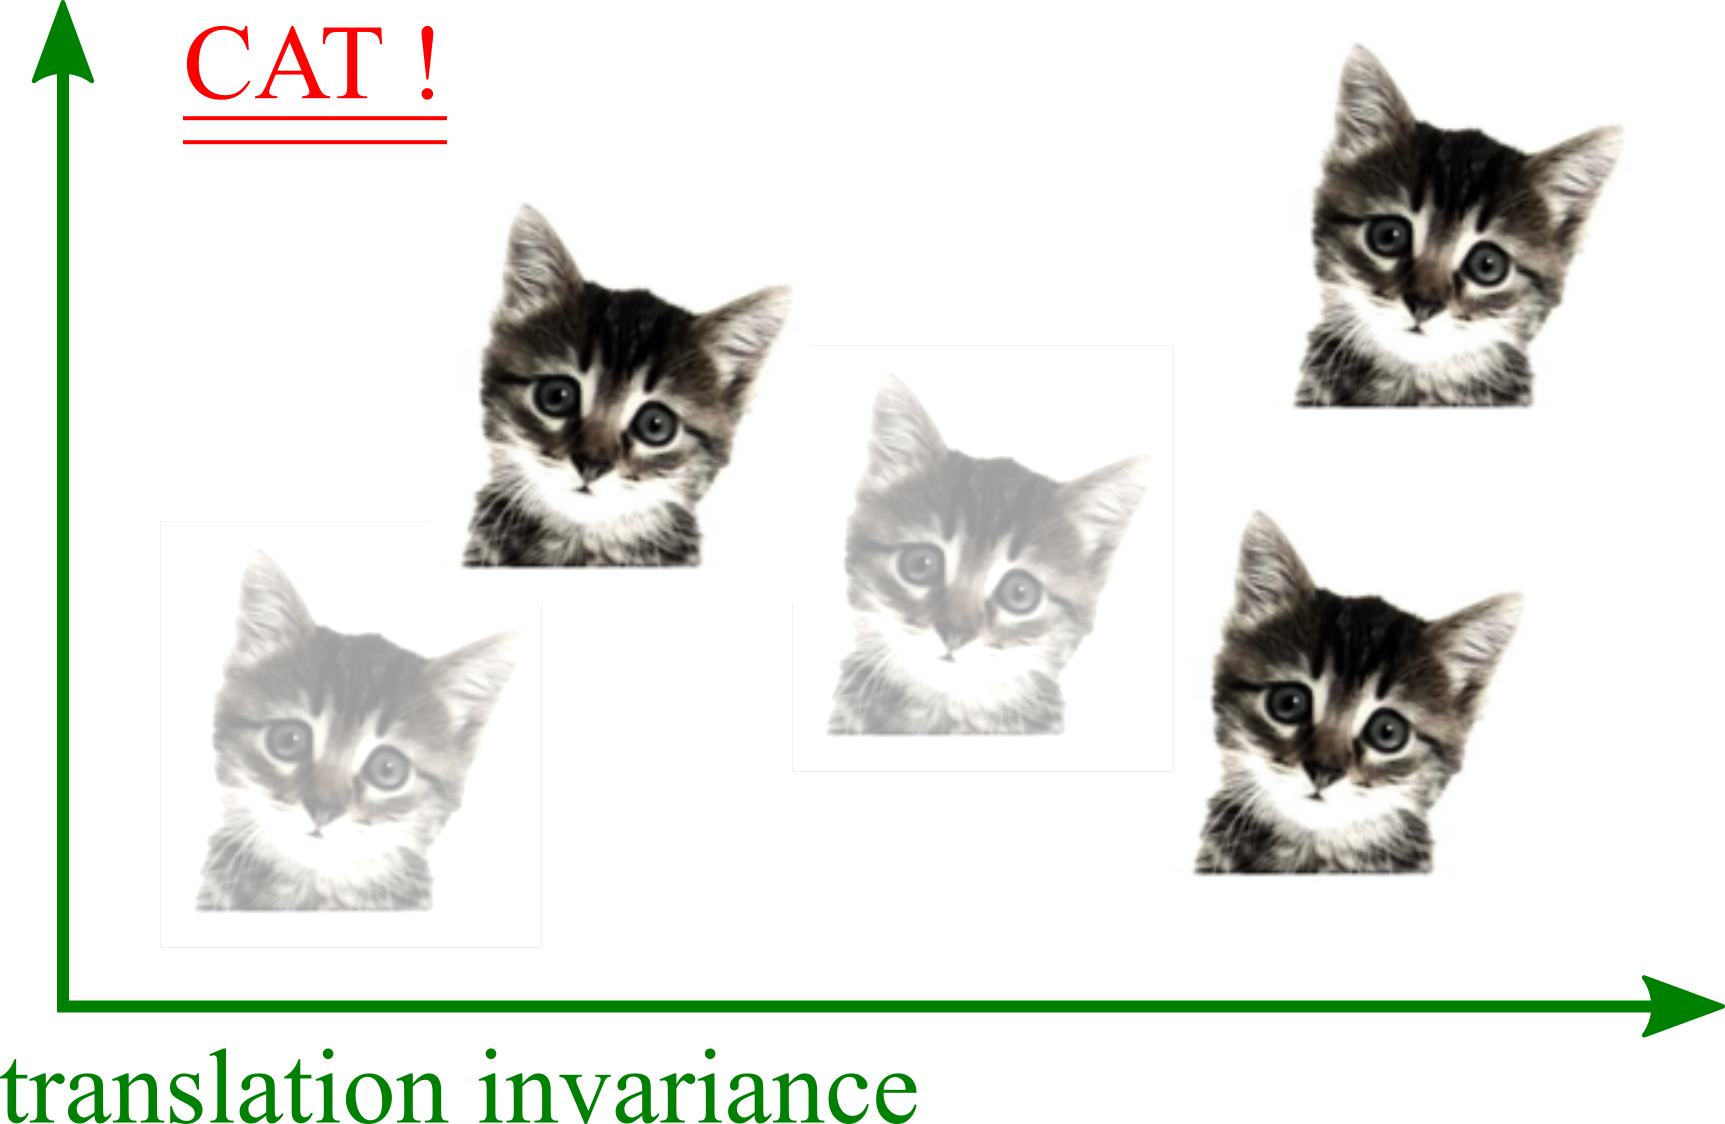
\includegraphics[scale=0.6]{translation-invariance.png}}}
	\end{equation}
	\item \cc{
	Convolution 是一种具有平移不变性的运算:}{
	\textbf{Convolution} is an operation invariant under translation:
	}
	\begin{equation}
	(T_x \circ f) * g = T_x \circ ( f * g )
	\end{equation}
\end{itemize}
\end{frame}

\begin{frame}[plain]
\begin{itemize}
	\item \cc{
	Yann LeCun 等人 利用 CNN 的 \emp{对称性} 加快了学习速度,成功地解决了 机器视觉 的问题}{
	Yann LeCun \textit{et al} exploited the symmetry of CNNs to accelerate learning, successfully solved the visual recognition problem
	}
	\begin{equation}
	\vcenter{\hbox{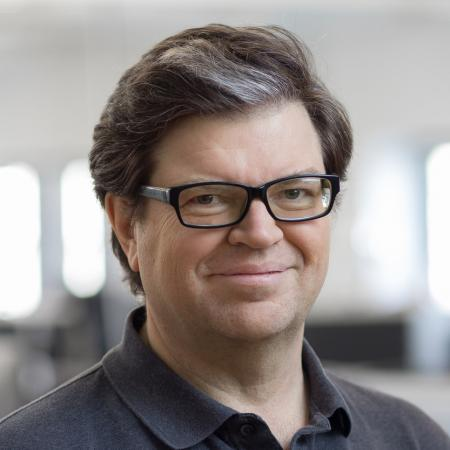
\includegraphics[scale=0.3]{Yann-LeCun.jpg}}}
	\end{equation}
\end{itemize}
\end{frame}

\begin{frame}
\frametitle{Symmetry and inductive bias}
\begin{itemize}
	\item \cc{
	在数学上,\emp{对称性} 经常能简化计算,所以数学家 特别喜欢 对称}{
	In mathematics, symmetry often simplifies computation, which is why mathematicians love to study symmetries
	}
	\item \cc{
	在机器学习中,经常要引入 归纳偏好 (inductive bias),缩小 \emp{搜寻空间}:}{
	In machine learning, one introduces \emp{inductive bias} to narrow down the \textbf{search space}:
	}
	\begin{equation}
	\vcenter{\hbox{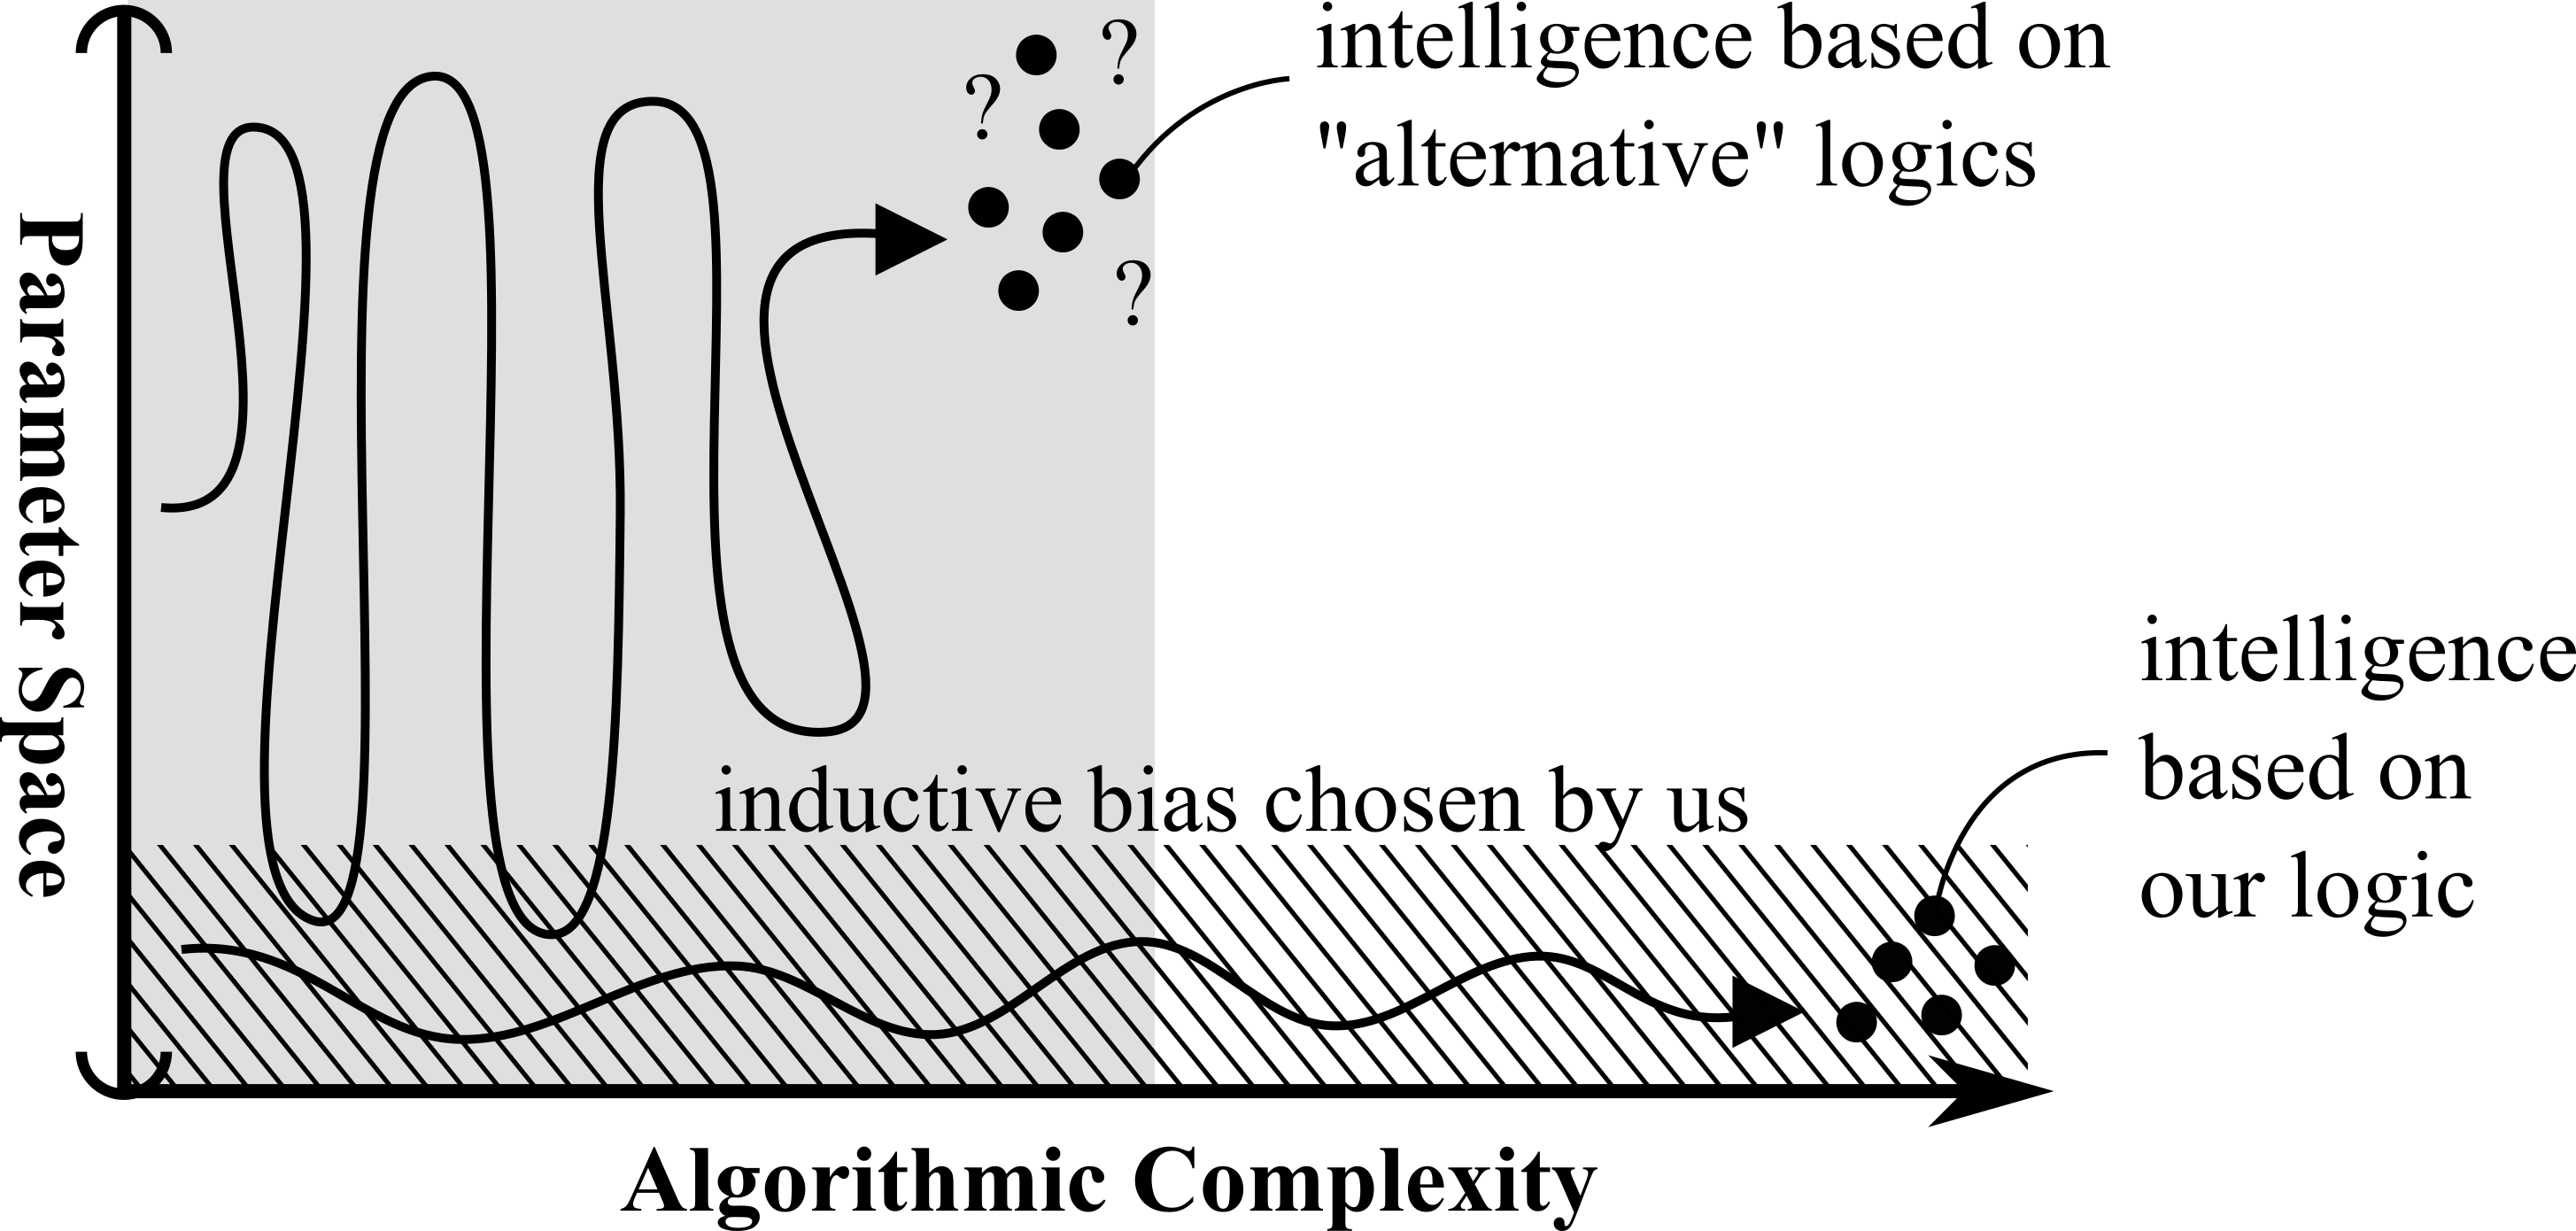
\includegraphics[scale=0.5]{no-free-lunch.png}}}
	\end{equation}
	\item \cc{
	往往如果 归纳偏好 选对了,可以在短时间内找到答案,否则问题是不可解的 (intractable)}{
	Oftentimes, if inductive bias is chosen correctly, solution is found quickly, otherwise problem becomes \textbf{intractable}
	}
\end{itemize}
\end{frame}

\begin{frame}
\frametitle{\cc{Richard Sutton 的观点}{Richard Sutton's view}}
\begin{itemize}
	\item \cc{
	Richard Sutton 认为,我们只需在 强化学习 的框架下 \emp{增加计算力},就可以找到 strong AI}{
	In contrast, Sutton expressed the view that AI can be solved merely by \textbf{increasing computing power}, under the reinforcement learning framework
	}
	\begin{equation}
	\vcenter{\hbox{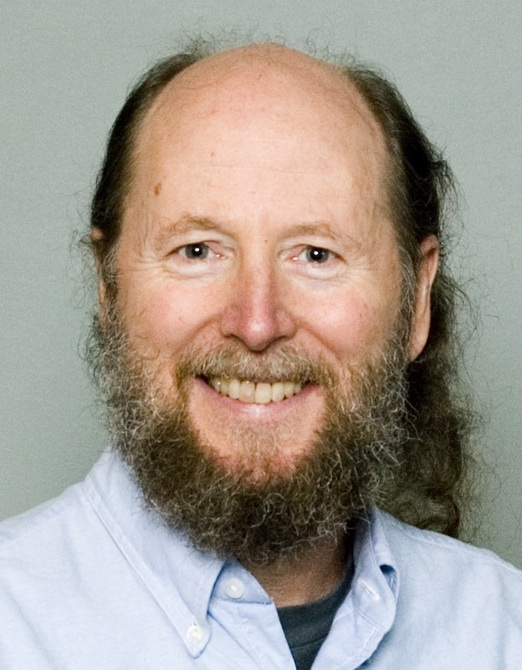
\includegraphics[scale=0.7]{Richard-Sutton.jpg}}}
	\end{equation}
\end{itemize}
\end{frame}

\begin{frame}[plain]
\begin{itemize}
	\item \cc{
	我們選擇的只是众多 形式逻辑 之中可能的一种:}{
	Our choice is just one out of many possible \textbf{forms} of logic:
	}
	\begin{equation}
	\vcenter{\hbox{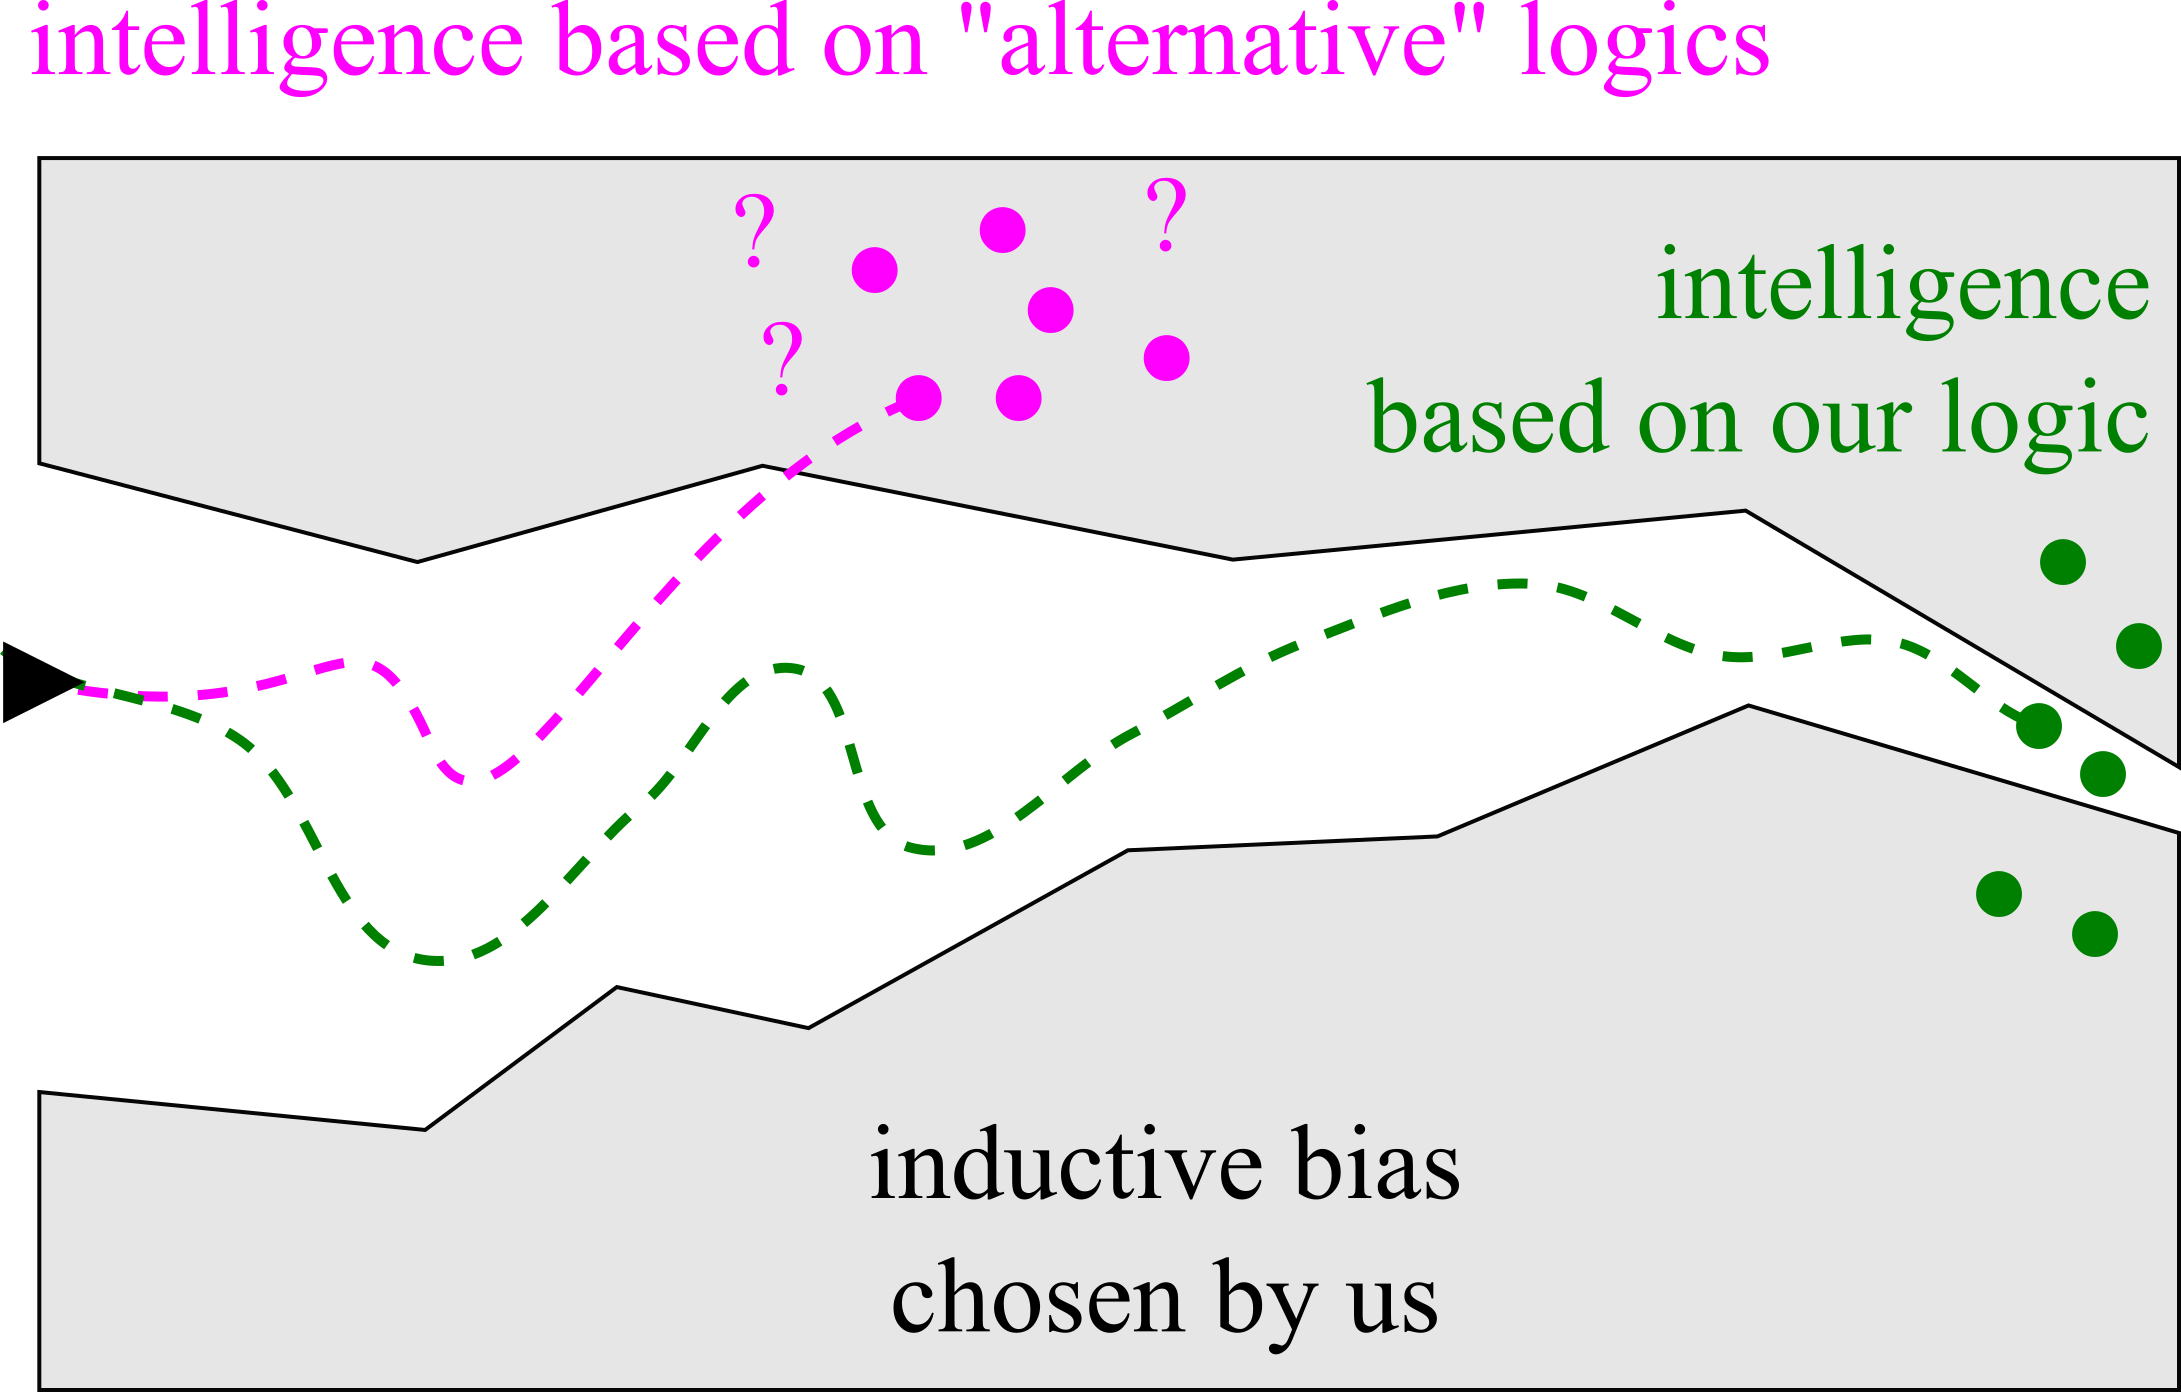
\includegraphics[scale=0.5]{no-free-lunch_Richard-Sutton.png}}}
	\end{equation}
	\item \cc{
	这不只是一个「空想」的问题; 事实上,世界各地的实验室 已经开始了对 AGI 不同形式的搜索!}{
	This is not only a theoretical issue; \\
	Indeed, AI labs around the world had begun the search for AGI with various strategies!
	}
\end{itemize}
\end{frame}

\begin{frame}
\frametitle{\cc{对 逻辑主义 的质疑}{Doubts about logicism}}
\begin{itemize}
	\item Admittedly, the human brain does \textbf{not} think like symbolic logic
	\item By symbolic logic, we mean any ``linear'' (sequential) representation
	\item In contrast, \textbf{pictures} and \textbf{music} are \textit{multi}-dimensional
	\item The brain may use representations that are not sequential or symbolic
	\item However, logic is a very efficient representation (from a computer perspective) even though it deviates from the biological brain
	\item Neuroscience is too difficult to crack, thus not a practical route to AGI
	% \item \cc{
	% 很多人怀疑: 人脑真的用 形式逻辑 思考吗?}{
	% Many are doubtful: does the human brain really use \textbf{formal logic} to think?
	% }
	% \item We tend to think there are ``little models'' inside our heads from which we draw inferences.
	\item \cc{其实人脑比我们想像中更接近逻辑}{
	Human cognition may be much closer to logic than we've thought.}
	If we're given a description:  ``woman finds new lover, murders husband'':
	\begin{equation}
	\vcenter{\hbox{
\includegraphics[scale=1.0]{murder-scene.png}}}
	\end{equation}
	We may not know:  Is the woman blonde? What is she wearing?
	In other words, our ``mental model'' is devoid of details and it may not possess any more information than just a sequence of symbols.
\end{itemize}
\end{frame}

\begin{frame}
\frametitle{Reinforcement learning}
\begin{itemize}
	\item Think of the ``\textbf{state}'' in reinforcement learning like a \textbf{board positon} in a chess game:
	\begin{equation}
	\vcenter{\hbox{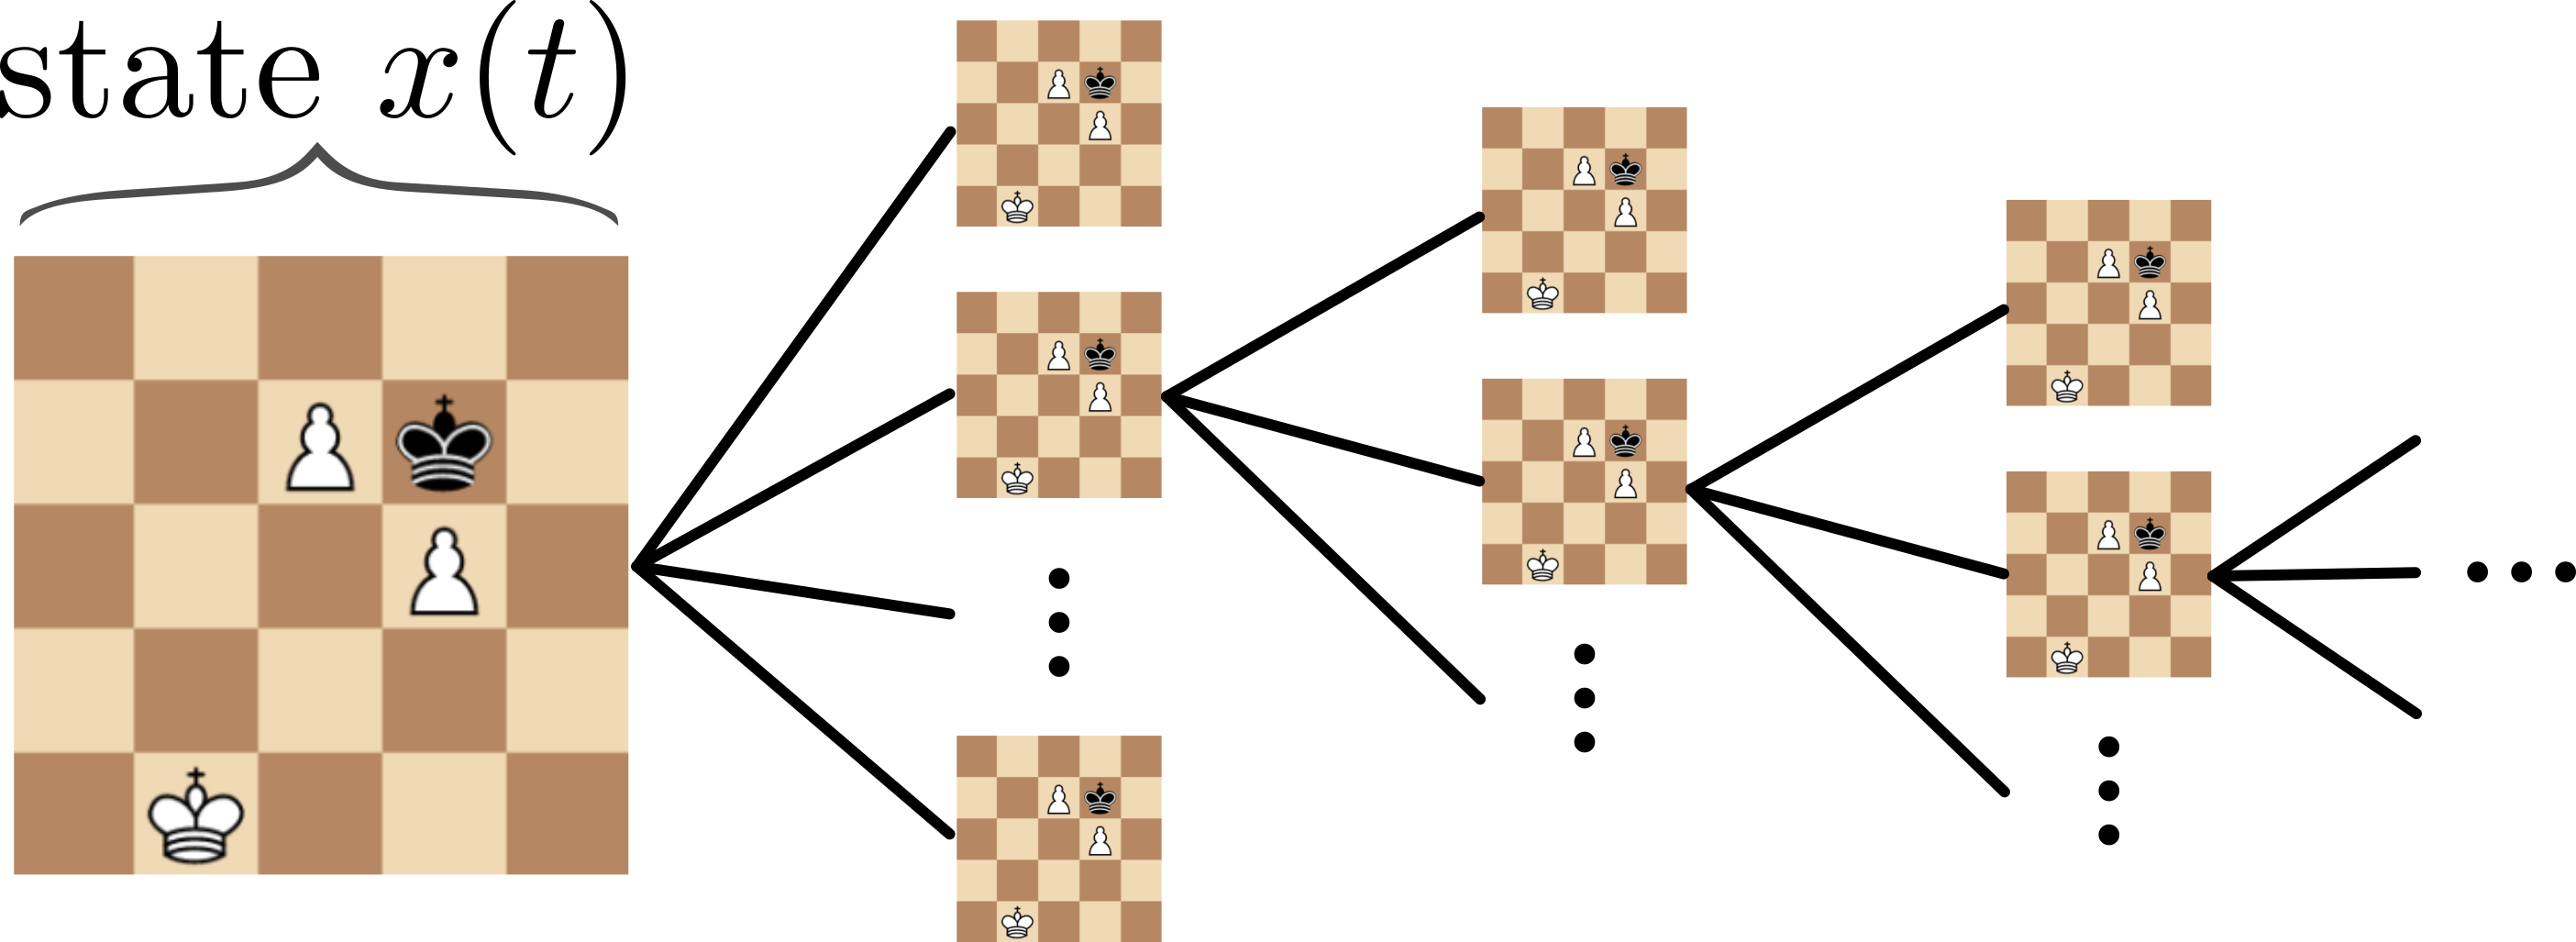
\includegraphics[scale=0.5]{chess-game-tree.png}}}
	\end{equation}
	\item Reinforcement learning seeks to maximize the total \textbf{rewards} accrued over a (possibly infinite) \textbf{time horizon}:
	\begin{equation}
	 \mbox{maximize }  S = \int_0^{\infty} L \; dt
	\end{equation}
	\item Such maximization gives the AI \textbf{intelligence} because it is often beneficial to \textbf{delay} rewards, eg: to plot a clever chess move
	\item But reinforcement learning is a \textbf{brute force} approach;  we need to give the model some additional \textbf{inductive bias}, eg, in the form of \textbf{logical structure}
\end{itemize}
\end{frame}

\begin{frame}
\frametitle{Structure of logic}
\begin{itemize}
	\item \cc{
	我的想法是: 在深度学习中引入 \emp{逻辑} 的对称性,解决 strong AI 问题}{
	The idea is:  introduce symmetries of \textbf{logic} into deep learning to solve the AGI problem
	}
	\item \cc{
	因为人的思维 具有 逻辑 的结构,这个 inductive bias 可以帮助我们快速找到 the solution to strong AI}{
	Because human cognition has logical structure, this inductive bias may help us find a solution to AGI faster
	}
	\item \cc{
	逻辑结构很复杂,但最粗略的 symmetry 是 命题的 \emp{可交换律} (commutativity, or permutation invariance):}{
	Logic is a complicated structure, but its simplest symmetry is the \textbf{commutativity} (or permutation invariance) of \textbf{propositions}:
	}
	\begin{equation}
	\begin{aligned}
	A &\wedge B & \equiv && B & \wedge A \\
	\mbox{\cc{下雨}{it's raining}} &\wedge \mbox{\cc{失恋}{lovesick}} & \equiv && \mbox{\cc{失恋}{lovesick}} &\wedge \mbox{\cc{下雨}{it's raining}}
	\end{aligned}
	\end{equation}
	\item \cc{
	它的重要性类似於 视觉中的 平移不变性}{
	Its importance may be analogous to translation invariance in vision
	}
	\item \cc{
	另一种讲法是: 它将智能系统的 \emp{思维状态} (mental state) 分拆成 一粒粒独立的 \emp{命题} (propositions)}{
	The significance of commutativity is:  it \textbf{decomposes} the AI system's \emp{mental state} into individual \emp{propositions}
	}
\end{itemize}
\end{frame}

\begin{frame}
\frametitle{Symmetric neural networks}
\begin{itemize}
	\item Permutation invariance can be handled by \emp{symmetric} neural networks

	\item \cc{我浪费了两年时间试图解决这问题,却发现在3年前已经有两篇论文解决了 [PointNet 2017] [DeepSets 2017],而且数学水平比我高很多
	}
	{I wasted 2 years trying to solve this problem, and then found out it had been solved 3 years before:  [PointNet 2017] and [DeepSets 2017] and their mastery of mathematics is significantly above me!}

	\item Any symmetric function can be represented by the following form (a special case of the Kolmogorov-Arnold representation of functions):
	\begin{equation}
	f(x, y, ...) = g(h(x) + h(y) + ... )
	\end{equation}
	\begin{equation}
	\vcenter{\hbox{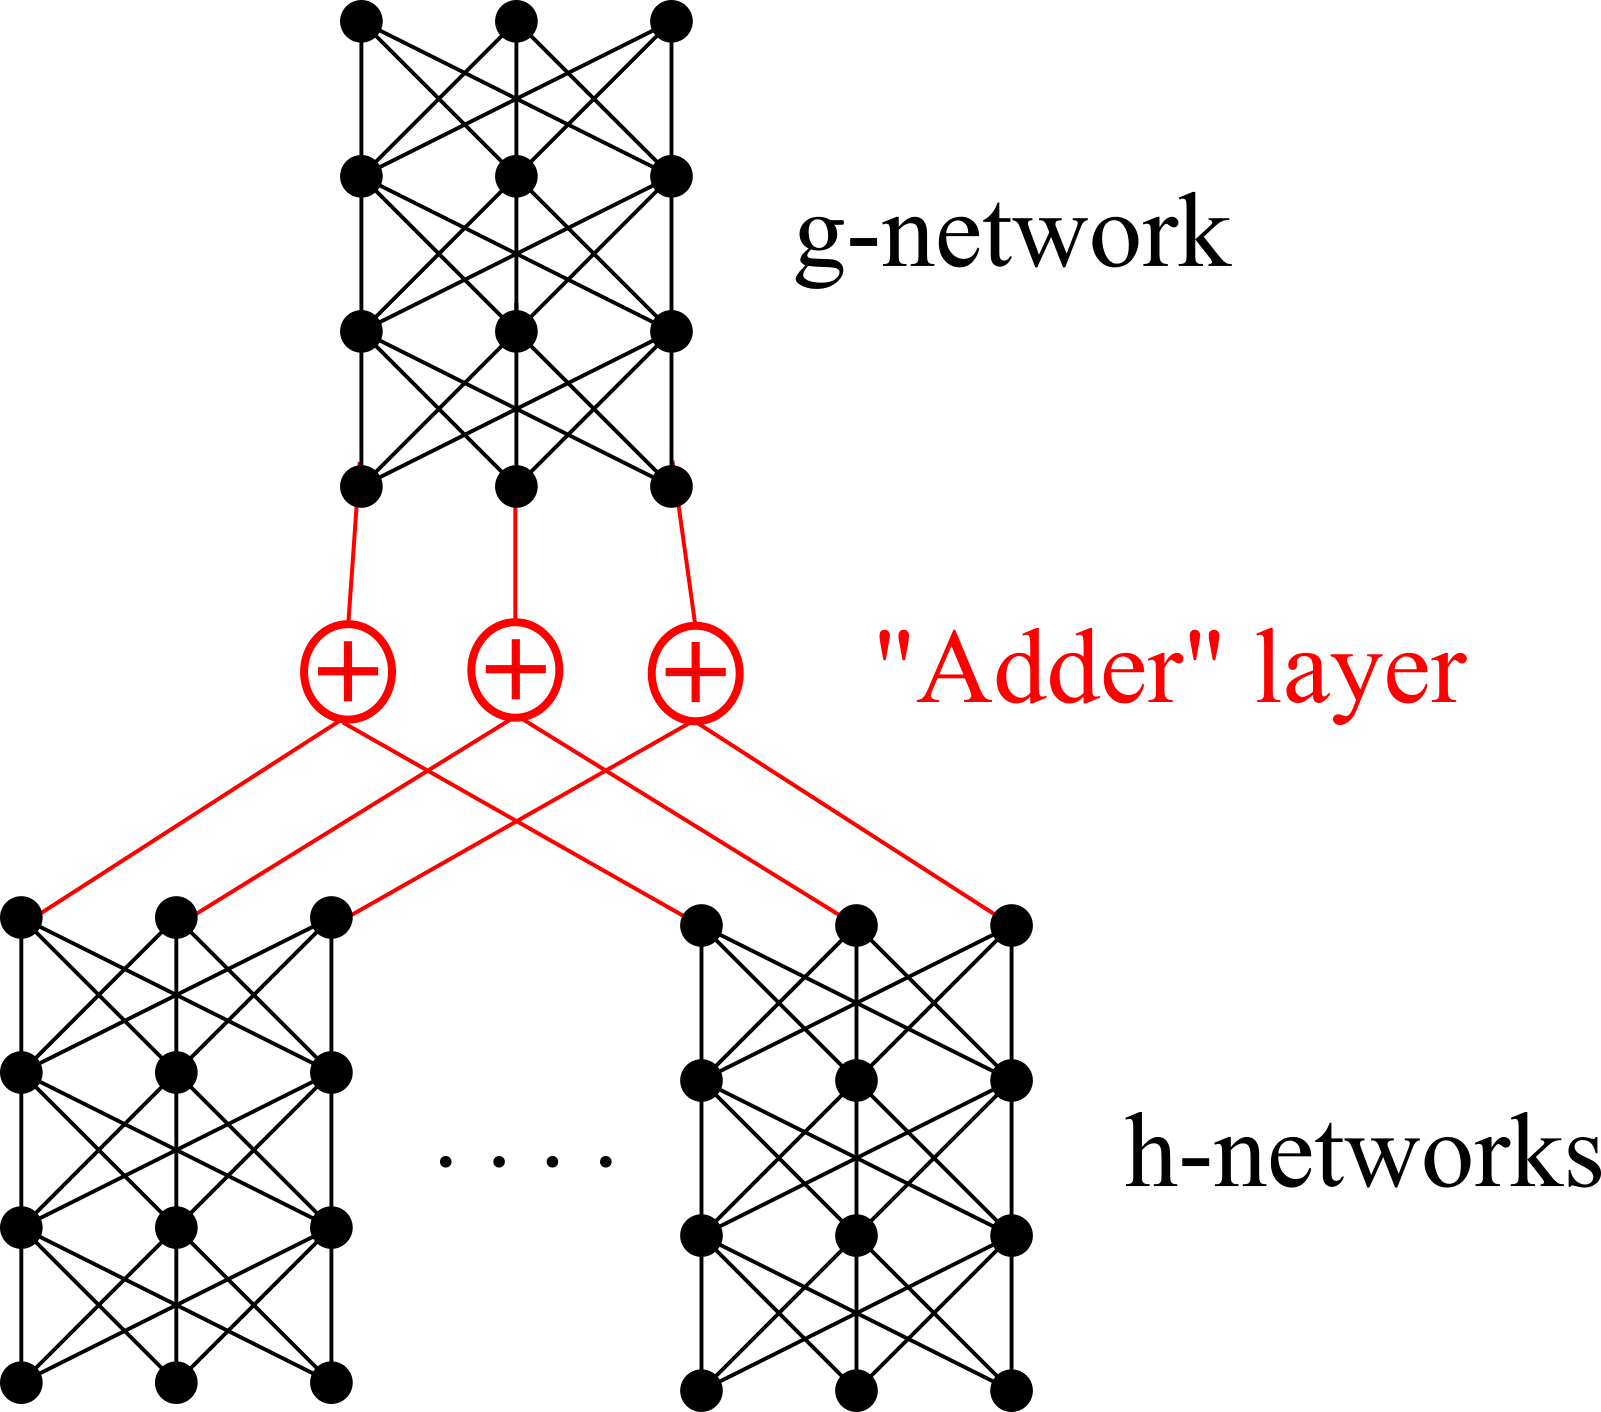
\includegraphics[scale=0.5]{g-and-h-networks.png}}}
	\end{equation}
\end{itemize}
\nocite{Qi2017a}
\nocite{Zaheer2017}
\end{frame}

\begin{frame}[plain]
\begin{itemize}
	\item Sym NN gives a powerful boost in efficiency $\propto n!$ where $n = \# \mbox{inputs}$

	\item The code for Sym NN is just a few lines of Tensorflow:
	\begin{equation}
	\vcenter{\hbox{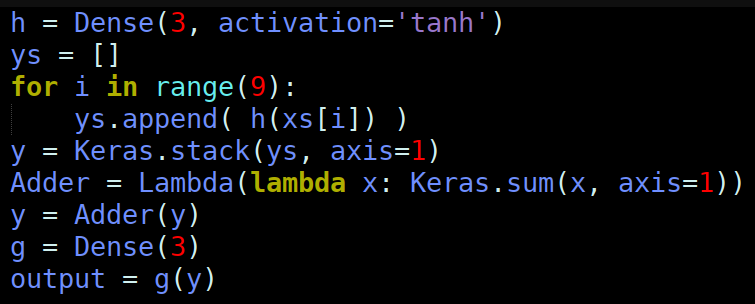
\includegraphics[scale=0.4]{sym-NN-code.png}}}
	\end{equation}
	\item Very easy to adopt this to existing models such as BERT and reinforcement learning
	\item I have successfully tested it on the game of TicTacToe: \\
	\href{https://github.com/Cybernetic1/policy-gradient}{https://github.com/Cybernetic1/policy-gradient}
\end{itemize}
\end{frame}

\begin{frame}
\frametitle{For example: symmetric NN for object recognition}
\begin{itemize}
	\item Imagine objects represented as \textbf{point clouds}:
		\begin{eqnarray}
		\nonumber
		\vcenter{\hbox{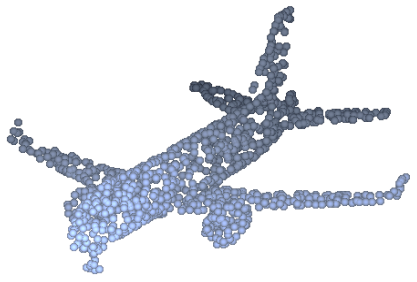
\includegraphics[scale=1]{point-cloud-aeroplane.png}}}
		\quad & \stackrel{f}{\longmapsto} & \quad \mbox{``aeroplane''} \\
		\nonumber
		\vcenter{\hbox{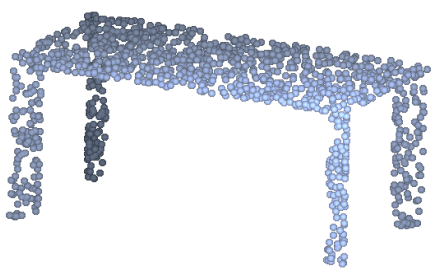
\includegraphics[scale=1]{point-cloud-desk.png}}}
		\quad & \stackrel{f}{\longmapsto} & \quad \mbox{``desk''}
		\end{eqnarray}
	\item It does not matter \textbf{in what order} the points are in a sequence; \\
		the function $f(x_1, ..., x_n)$ is symmetric in its arguments (the points)
	\item Permutation invariance is \textbf{essential} for this to work
\end{itemize}
\end{frame}

\renewcommand{\baselinestretch}{0.9} 
\begin{frame}
\frametitle{\cc{BERT 的逻辑化}{Logicalization of BERT}}
\begin{itemize}
	\item \cc{类似地,可以将 BERT 的 隐状态 变成 ``set of propositions'' 的形式,方法是将 原来的 decoder 变成 sym NN:}
	{Similarly, we can convert BERT's hidden state into a set of propositions, by replacing the original \emp{decoder} with a sym NN:}
	\begin{equation}
	\vcenter{\hbox{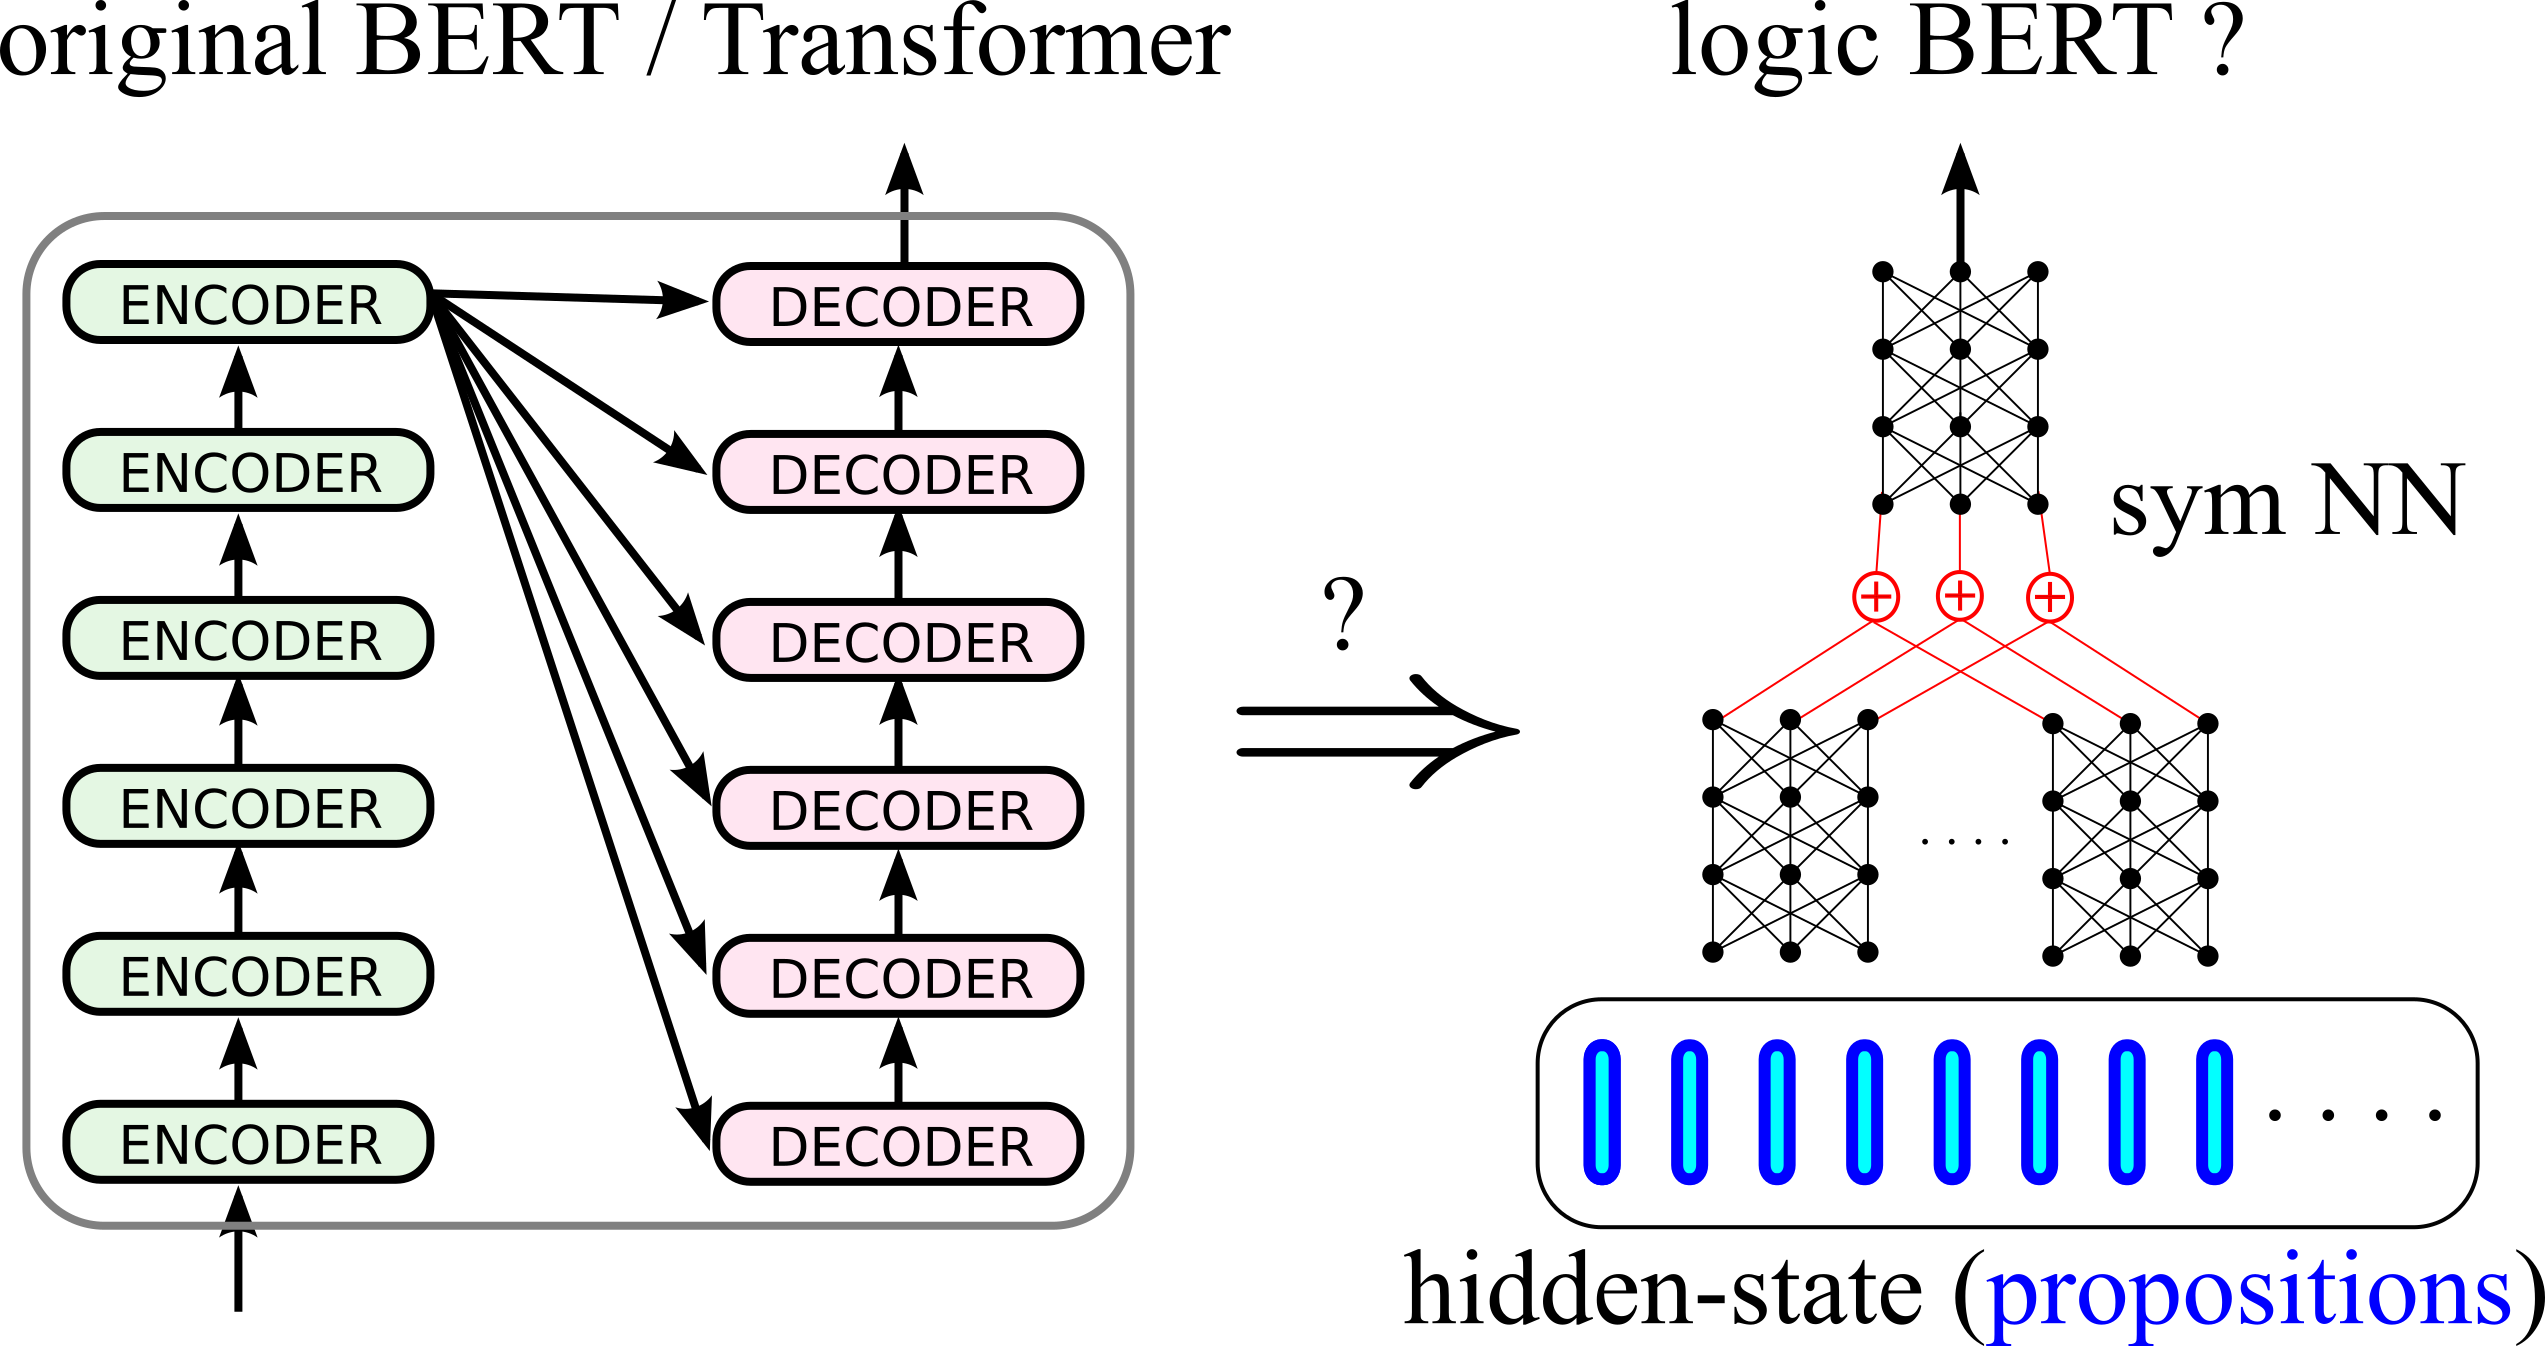
\includegraphics[scale=0.6]{sym-BERT.png}}}
	\end{equation}
	\item \cc{原来的 encoder 可以照旧使用,因为后半部改变了,error propagation 会令 representation 也改变}
	{The original \emp{encoder} can be retained.  As the \emp{decoder} imposes symmetry on the hidden state, error propagation is expected to cause its representation to change}
	\item \cc{当然,这个想法有待实验证实 \smiley}
	{Of course, this remains to be proven by experiment \smiley}
\end{itemize}
\end{frame}
\renewcommand{\baselinestretch}{1.0} 

\begin{frame}
\frametitle{Advantages of logical AI (1)}
\begin{itemize}
	% \item \cc{以前 BERT 的隐状态 没有逻辑结构,我们不是很清楚它的内容是什么; 逻辑化之后,BERT 内部的命题可以储存在 \emp{长期记忆} 中:}
	% {The original BERT hidden state lacked a logical structure and it was not clear what exactly it contains.  After logicalization, propositions inside BERT can be stored into \emp{long-term memory}:}
	\item With logic, it becomes easy to design cognitive architectures, \\
	eg: long-term memory module
	\begin{equation}
	\vcenter{\hbox{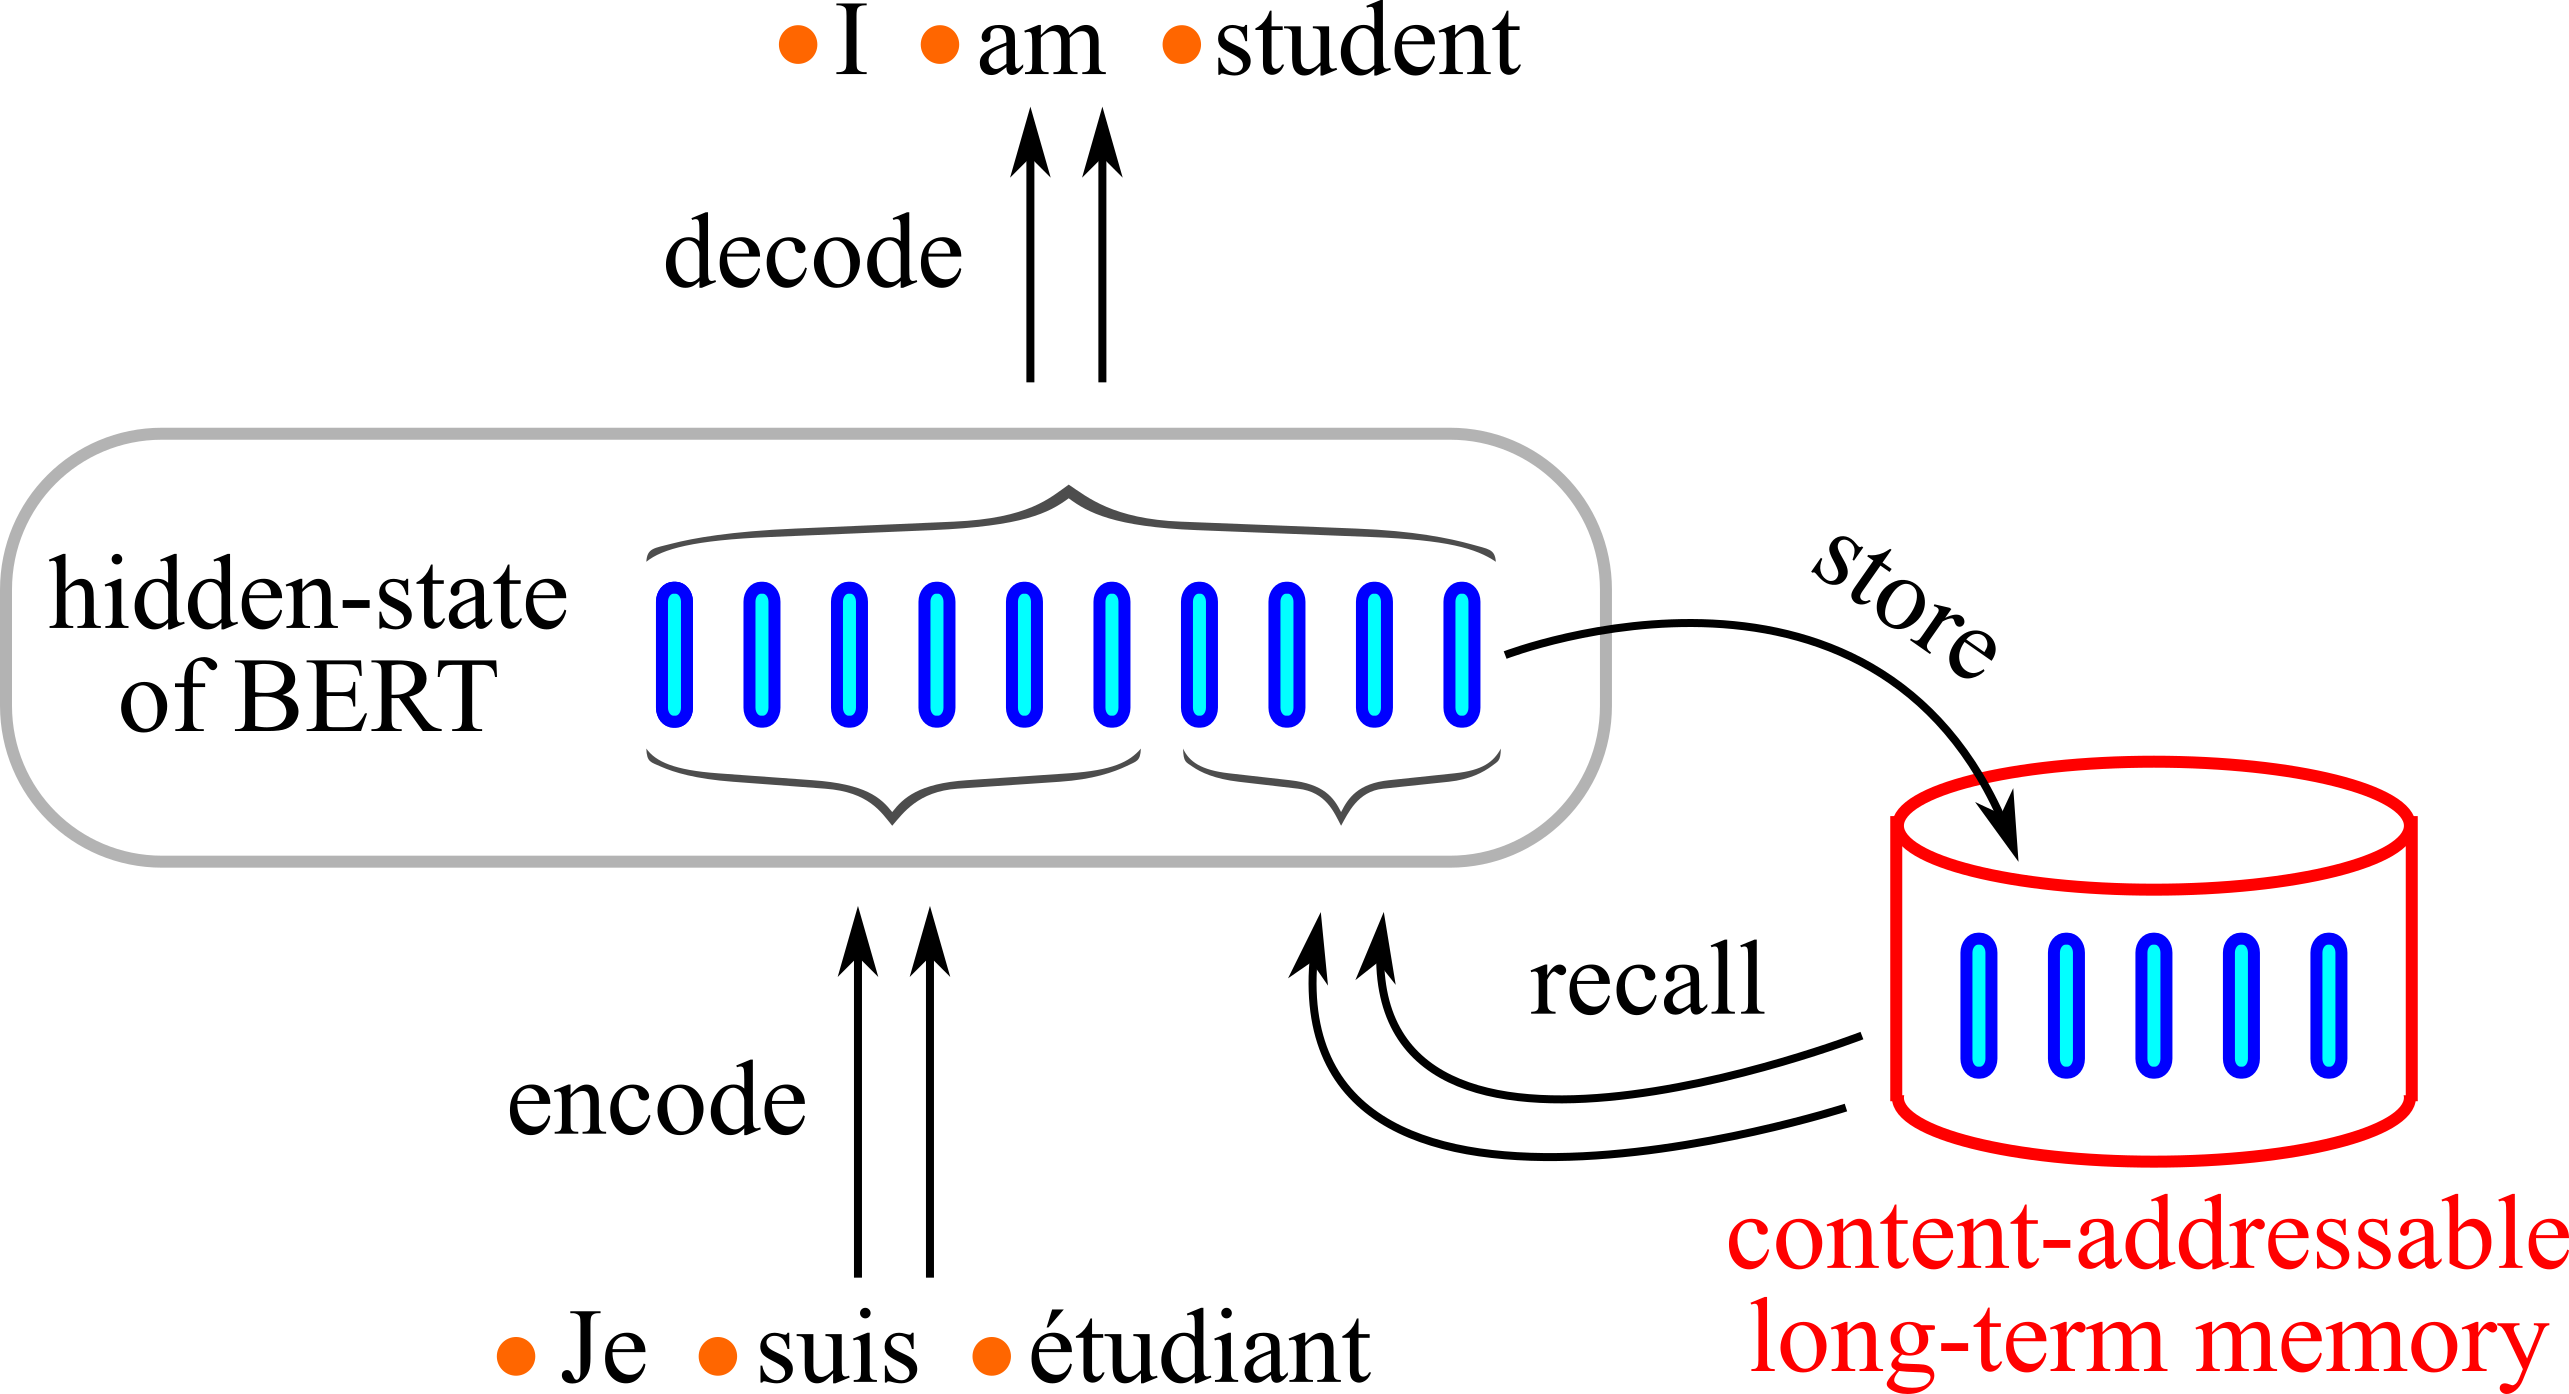
\includegraphics[scale=0.5]{long-term-memory.png}}}
	\end{equation}
	% 例如:「太阳是热的」、「水向下流」是经常正确的命题
	% \item \cc{这种系统 已非常接近 strong AI,而这是有赖 \emp{逻辑化} 才能做到的}
	% {These kind of systems are very close to strong AI, and it depends crucially on logicalization}
	% \item \cc{Content-addressable memory 的想法来自 Alex Graves \textit{et al} 的 Neural Turing Machine [2014]}
	% {The content-addressable memory idea came from Alex Graves \textit{et al}'s Neural Turing Machine [2014]}
 \end{itemize}
% \nocite{Graves2014}
\end{frame}

\begin{frame}
\frametitle{Advantages of logical AI (2)}
\begin{itemize}
	\item \cc{知识图谱 不能直接输入神经网络,它必需分拆成很多 edges,每个 edge 是一个 \emp{关系},也是一个 \emp{逻辑命题} ;也可以说 ``graphs are isomorphic to logic''}
	% {One cannot feed a knowledge graph directly into an NN, as its input must be embedded in vector space.  A solution is to break the graph into edges, where each edge is equivalent to a relation or proposition.  One could say that graphs are isomorphic to logic}
	{Integrate seamlessly with \emp{knowledge graphs}}
	\item graphs are made up of edges, \\
	edges = relations between nodes = propositions:
	\begin{equation}
	\vcenter{\hbox{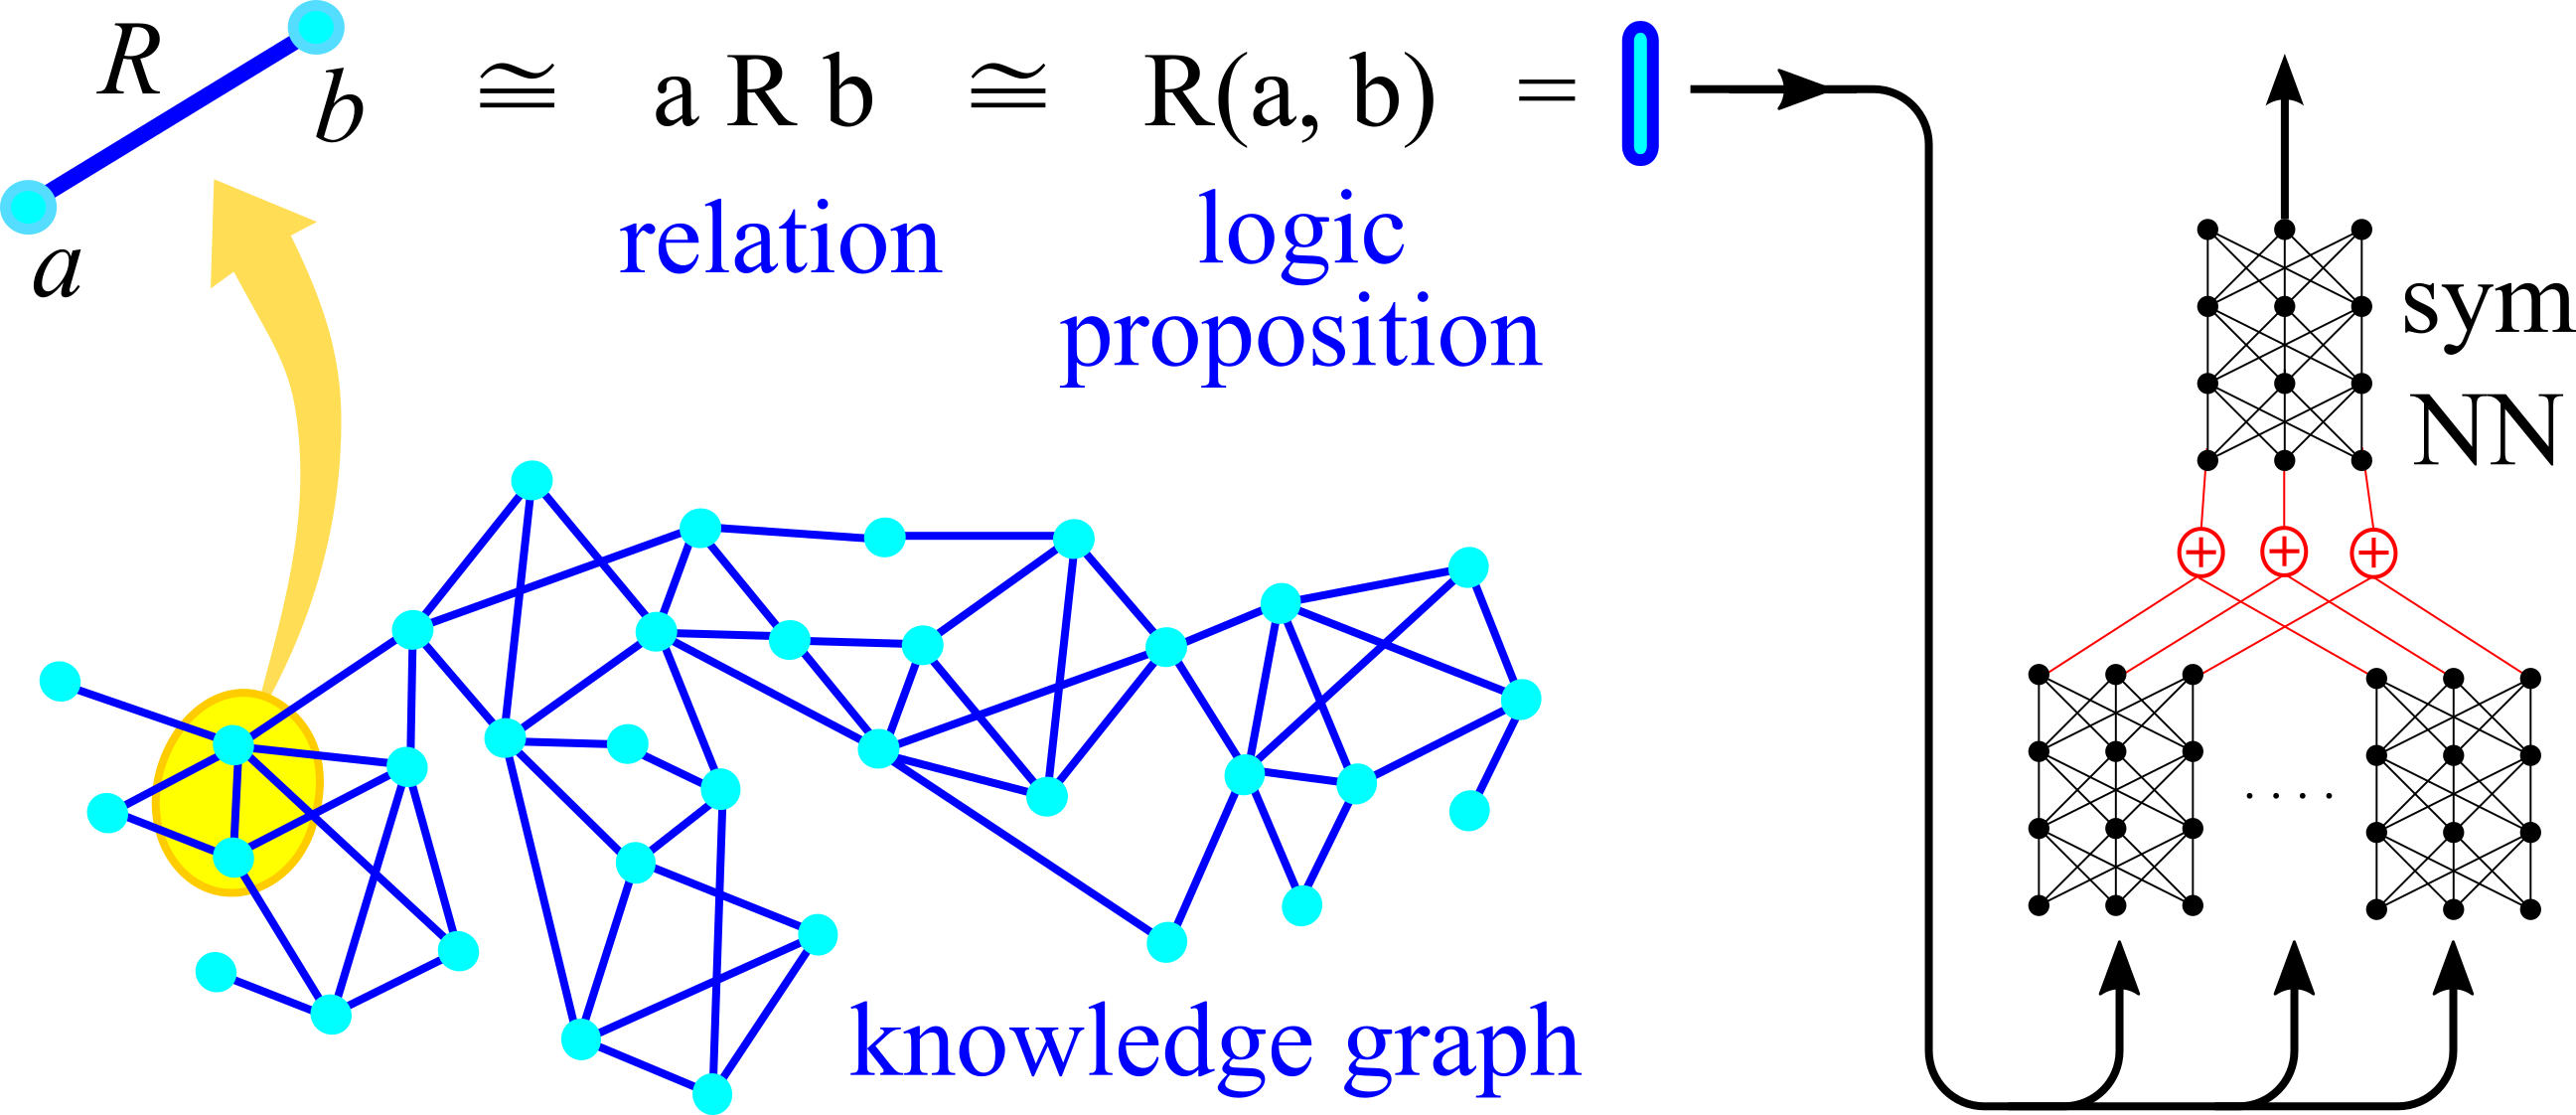
\includegraphics[scale=0.6]{knowledge-graph.png}}}
	\end{equation}
	% \item \cc{而这些 edges 似乎必需用 \emp{symmetric} NN 处理,因为它们是 permutation invariant}
	% {Since edges are invariant under permutations, it appears that symmetric NNs are required to process them}
	% \item Sym NNs are required to handle \emp{graph-rewriting}, an essential operation on knowledge graphs
\end{itemize}
\end{frame}

%\begin{frame}
%\frametitle{AGI 理论的突破}
%\begin{itemize}
%	\item 最近我成功地描述了 strong AI 和 逻辑之间的数学关系 \\
%	这种数学关系是永恒不变的,它可以指导日后 AGI 的发展 \\
%	请参看附件:《再谈一次 AI 的逻辑结构》
%	
%	\item 关於 Logic BERT 与 attention 的详细理论 \\
%	可参看附件《Logic BERT》
%\end{itemize}
%\end{frame}

%\begin{frame}
%\frametitle{再谈一次 逻辑结构}
%\begin{itemize}
%	\item 我发现 逻辑 和 AI 之间 有很漂亮的理论
%	\item 现代逻辑理论 揭示出某些 \emp{几何} (geometry) 与 \emp{拓樸} (topology) 结构
%	\item 大家 中/小学 时期 都熟悉 Venn diagrams,其实 命题逻辑 具有 \emp{拓扑}结构:
%	\begin{equation}
%	\vcenter{\hbox{\includegraphics[scale=0.4]{Venn-diagram.png}}}
%	\end{equation}
%	而 谓词 (predicates) 是在 base set 上面的 纤维化 (fibration), 记作 $\mathrel{\substack{\mathbb{E}\\\downarrow \\\mathbb{B}}  {\scriptstyle p}}$
%
%	\item 另方面,著名的 Curry-Howard isomorphism 揭示 \emp{逻辑证明} 与 \emp{编程语言} 之间的深刻关系:
%	\begin{eqnarray}
%	\mbox{逻辑} & \Leftrightarrow & \mbox{type theory} \\
%	\mbox{逻辑证明} & \Leftrightarrow & \mbox{programs} \nonumber
%	\end{eqnarray}
%	\item 程式 是一些 \emp{函数},而 神经网络 也是非线性的函数\emp{映射},所以 神经网络 也\emp{对应于} 逻辑推理
%\end{itemize}
%\end{frame}

%\begin{frame}[fragile]
%\begin{itemize}
%	\item BERT 似乎是在执行 句子之间的变换,而这些句子是 word embedding 的 concatenation,例如:
%	\begin{equation}
%	\begin{tikzcd}[column sep = large]
%	\mbox{苏格拉底} \cdot \mbox{是} \cdot \mbox{人}
%	\arrow[r, "BERT"]
%	& \mbox{苏格拉底} \cdot \mbox{会} \cdot \mbox{死}
%	\end{tikzcd}
%	\end{equation}
%	这个做法看似很「粗暴」,其实它和逻辑式子的作用一样:
%	\begin{equation}
%	\forall x. \; \mbox{Human}(x) \rightarrow \mbox{Mortal}(x)
%	\end{equation}
%	而这式子,根据 Curry-Howard 对应,就是上面的函数映射!
%	
%	\item 这些映射的对象,是形如 ``$a \in A$'' 这样的物体,它们有 predicates 的几何/拓扑结构,但我们现时未做到这一步,暂时只引入了 commutativity

	% \item 集合元素 $a$ 是 $\exists x. P(x)$ 的证明,例如 Socrates 是 $\exists x. \mbox{mortal}(x)$ 的证明
	% \item 当 神经网络 \emp{调教} 某些元素的 映射 (mapping) 时,它同时在学习某个逻辑的 formula;  换句话说,逻辑 是几何空间中的映射
	% \item 逻辑的 谓词 (predicates) 是在 基底元素空间上的一个 \emp{纤维丛结构} (fibration) :
	%\begin{equation}
	%\vcenter{\hbox{\includegraphics[scale=0.5]{etale-space.png}}}
	%\end{equation}
%	\item 从 几何/拓扑 ``借'' 来的概念,演变成 topos 理论、HoTT (homotopy type theory) 等
%	\item 这些漂亮的理论 不是无用的; 有需要时,可以從 邏輯 那邊借來更多的結構
%\end{itemize}
%\end{frame}

\frameinlbffalse
\begin{frame}
\frametitle{References}
\cc{多谢收看}{Thanks for watching} \smiley \\
% \printbibliography
\textbf{Illustration credits:}
\begin{itemize}
	\item Translation invariance, from Udacity Course 730, Deep Learning (L3 Convolutional Neural Networks $\rhd$ Convolutional Networks)
	% \item \'{E}tale space, from Topoi -- The Categorical Analysis of Logic [Goldblatt 2006]
\end{itemize}
\end{frame}

\end{document} 